% =========================================
% Erciyes Üniversitesi Kampüs Ağı Tasarımı
% University Campus Network Design Project
% LaTeX Documentation
% =========================================
\documentclass[12pt,a4paper]{article}

% --- Packages ---
\usepackage[utf8]{inputenc}
\usepackage[T1]{fontenc}
\usepackage[shorthands=:!,turkish,english]{babel}
\usepackage{geometry}
\usepackage{graphicx}
\usepackage{xcolor}
\usepackage{tikz}
\usepackage{listings}
\usepackage{hyperref}
\usepackage{fancyhdr}
\usepackage{titlesec}
\usepackage{booktabs}
\usepackage{longtable}
\usepackage{array}
\usepackage{caption}
\usepackage{subcaption}
\usepackage{float}
\usepackage{enumitem}
\usepackage{tcolorbox}
\usepackage{amsmath}
\usepackage{tabularx}

% TikZ Libraries
\usetikzlibrary{shapes.geometric, shapes.symbols, shapes.misc, arrows.meta, positioning, fit, calc, backgrounds, decorations.pathreplacing}

% --- Page Geometry ---
\geometry{
  top=2.5cm,
  bottom=2.5cm,
  left=2.5cm,
  right=2.5cm
}

% --- Colors ---
\definecolor{erciyesred}{RGB}{153, 0, 0}
\definecolor{ciscoblue}{RGB}{0, 86, 150}
\definecolor{darkgreen}{RGB}{0, 100, 0}
\definecolor{codebg}{RGB}{245, 245, 245}
\definecolor{codeframe}{RGB}{200, 200, 200}
\definecolor{corekw}{RGB}{0, 0, 180}
\definecolor{accessgreen}{RGB}{34, 139, 34}
\definecolor{distblue}{RGB}{70, 130, 180}
\definecolor{corered}{RGB}{200, 50, 50}

% --- Cisco IOS Listings Style ---
\lstdefinestyle{cisco}{
  backgroundcolor=\color{codebg},
  frame=single,
  rulecolor=\color{codeframe},
  basicstyle=\ttfamily\footnotesize,
  keywordstyle=\color{corekw}\bfseries,
  commentstyle=\color{darkgreen}\itshape,
  stringstyle=\color{erciyesred},
  breaklines=true,
  breakatwhitespace=false,
  numbers=left,
  numberstyle=\tiny\color{gray},
  numbersep=8pt,
  showstringspaces=false,
  tabsize=2,
  captionpos=b,
  morekeywords={hostname, enable, configure, terminal, interface, ip, address, no, shutdown,
    switchport, mode, trunk, access, vlan, voice, exit, router, ospf, network, area,
    standby, version, priority, preempt, helper-address, channel-group, port-security,
    crypto, isakmp, ipsec, transform-set, map, set, peer, match, encapsulation, dot1Q,
    telephony-service, ephone-dn, number, nat, inside, outside, source, list, overload,
    access-list, permit, deny, any, spanning-tree, portfast, bpduguard, password, login,
    secret, banner, motd, service, password-encryption, username, ssh, transport, input,
    access-class, line, vty, console, range, description, write, memory, routing,
    default-router, option, dns-server, pool, excluded-address, dhcp, route, log-adjacency-changes,
    max-ephones, max-dn, auto, assign, key, policy, encryption, aes, authentication,
    pre-share, group, esp-aes, esp-sha-hmac, ipsec-isakmp, sticky, maximum, violation,
    mac-address, name, do, wr, conf, gigabitEthernet, fastEthernet, serial, Port-channel},
  morecomment=[l]{!},
  literate={ı}{{\i}}1 {İ}{{\.{I}}}1 {ö}{{\"o}}1 {Ö}{{\"O}}1 {ü}{{\"u}}1 {Ü}{{\"U}}1
           {ş}{{\c{s}}}1 {Ş}{{\c{S}}}1 {ç}{{\c{c}}}1 {Ç}{{\c{C}}}1 {ğ}{{\u{g}}}1 {Ğ}{{\u{G}}}1
}

% --- Header/Footer ---
\pagestyle{fancy}
\fancyhf{}
\fancyhead[L]{\small\textcolor{erciyesred}{Erciyes Üniversitesi -- Bilgisayar Mühendisliği}}
\fancyhead[R]{\small\textcolor{ciscoblue}{Kampüs Ağı Tasarımı}}
\fancyfoot[C]{\thepage}
\renewcommand{\headrulewidth}{0.4pt}
\renewcommand{\footrulewidth}{0.4pt}

% --- Section Formatting ---
\titleformat{\section}
  {\Large\bfseries\color{erciyesred}}
  {\thesection}{1em}{}
\titleformat{\subsection}
  {\large\bfseries\color{ciscoblue}}
  {\thesubsection}{1em}{}
\titleformat{\subsubsection}
  {\normalsize\bfseries\color{darkgreen}}
  {\thesubsubsection}{1em}{}

% --- Hyperlinks ---
\hypersetup{
  colorlinks=true,
  linkcolor=erciyesred,
  urlcolor=ciscoblue,
  citecolor=darkgreen,
  pdftitle={Erciyes Üniversitesi - Kampüs Ağı Tasarımı},
  pdfauthor={Berkay Aydemir},
}

% --- TCoBox for Info Boxes ---
\newtcolorbox{infobox}[1][]{
  colback=blue!5!white,
  colframe=ciscoblue,
  fonttitle=\bfseries,
  title=#1
}

\newtcolorbox{warningbox}[1][]{
  colback=red!5!white,
  colframe=erciyesred,
  fonttitle=\bfseries,
  title=#1
}

% =========================================
% DOCUMENT BEGIN
% =========================================
\begin{document}

% --- Title Page ---
\begin{titlepage}
  \centering
  \vspace*{1cm}

  {\Large\textbf{2025--2026 AKADEMİK YILI -- GÜZ DÖNEMİ}}

  \vspace{1.5cm}

  \rule{\textwidth}{1.5pt}
  \vspace{0.5cm}

  {\Huge\bfseries\textcolor{erciyesred}{Üniversite Kampüs Ağı\\Tasarımı Projesi}}

  \vspace{0.3cm}
  {\Large\textcolor{ciscoblue}{University Campus Network Design}}

  \vspace{0.5cm}
  \rule{\textwidth}{1.5pt}

  \vspace{2cm}

  % --- TikZ Network Icon ---
  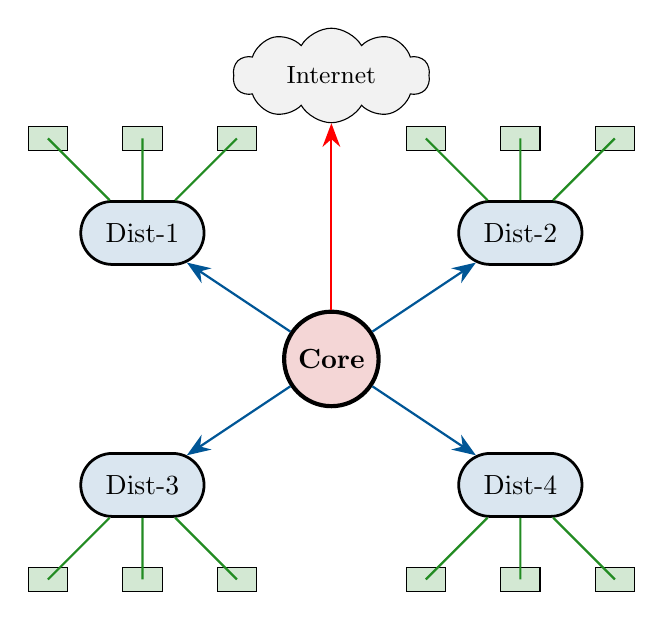
\begin{tikzpicture}[scale=0.8]
    % Central router
    \node[draw, circle, minimum size=1.2cm, fill=corered!20, line width=1.5pt] (core) at (0,0) {\textbf{Core}};

    % Distribution switches
    \node[draw, rounded rectangle, minimum width=1.8cm, minimum height=0.8cm, fill=distblue!20, line width=1pt] (d1) at (-3,2) {Dist-1};
    \node[draw, rounded rectangle, minimum width=1.8cm, minimum height=0.8cm, fill=distblue!20, line width=1pt] (d2) at (3,2) {Dist-2};
    \node[draw, rounded rectangle, minimum width=1.8cm, minimum height=0.8cm, fill=distblue!20, line width=1pt] (d3) at (-3,-2) {Dist-3};
    \node[draw, rounded rectangle, minimum width=1.8cm, minimum height=0.8cm, fill=distblue!20, line width=1pt] (d4) at (3,-2) {Dist-4};

    % Access layer
    \node[draw, rectangle, minimum width=0.5cm, minimum height=0.3cm, fill=accessgreen!20] at (-4.5,3.5) {};
    \node[draw, rectangle, minimum width=0.5cm, minimum height=0.3cm, fill=accessgreen!20] at (-3,3.5) {};
    \node[draw, rectangle, minimum width=0.5cm, minimum height=0.3cm, fill=accessgreen!20] at (-1.5,3.5) {};
    \node[draw, rectangle, minimum width=0.5cm, minimum height=0.3cm, fill=accessgreen!20] at (1.5,3.5) {};
    \node[draw, rectangle, minimum width=0.5cm, minimum height=0.3cm, fill=accessgreen!20] at (3,3.5) {};
    \node[draw, rectangle, minimum width=0.5cm, minimum height=0.3cm, fill=accessgreen!20] at (4.5,3.5) {};
    \node[draw, rectangle, minimum width=0.5cm, minimum height=0.3cm, fill=accessgreen!20] at (-4.5,-3.5) {};
    \node[draw, rectangle, minimum width=0.5cm, minimum height=0.3cm, fill=accessgreen!20] at (-3,-3.5) {};
    \node[draw, rectangle, minimum width=0.5cm, minimum height=0.3cm, fill=accessgreen!20] at (-1.5,-3.5) {};
    \node[draw, rectangle, minimum width=0.5cm, minimum height=0.3cm, fill=accessgreen!20] at (1.5,-3.5) {};
    \node[draw, rectangle, minimum width=0.5cm, minimum height=0.3cm, fill=accessgreen!20] at (3,-3.5) {};
    \node[draw, rectangle, minimum width=0.5cm, minimum height=0.3cm, fill=accessgreen!20] at (4.5,-3.5) {};

    % Connections
    \draw[-{Stealth[length=3mm]}, thick, ciscoblue] (core) -- (d1);
    \draw[-{Stealth[length=3mm]}, thick, ciscoblue] (core) -- (d2);
    \draw[-{Stealth[length=3mm]}, thick, ciscoblue] (core) -- (d3);
    \draw[-{Stealth[length=3mm]}, thick, ciscoblue] (core) -- (d4);

    \draw[thick, accessgreen] (d1) -- (-4.5,3.5);
    \draw[thick, accessgreen] (d1) -- (-3,3.5);
    \draw[thick, accessgreen] (d1) -- (-1.5,3.5);
    \draw[thick, accessgreen] (d2) -- (1.5,3.5);
    \draw[thick, accessgreen] (d2) -- (3,3.5);
    \draw[thick, accessgreen] (d2) -- (4.5,3.5);
    \draw[thick, accessgreen] (d3) -- (-4.5,-3.5);
    \draw[thick, accessgreen] (d3) -- (-3,-3.5);
    \draw[thick, accessgreen] (d3) -- (-1.5,-3.5);
    \draw[thick, accessgreen] (d4) -- (1.5,-3.5);
    \draw[thick, accessgreen] (d4) -- (3,-3.5);
    \draw[thick, accessgreen] (d4) -- (4.5,-3.5);

    % Internet cloud
    \node[draw, cloud, cloud puffs=10, cloud puff arc=120, aspect=2.5,
          minimum width=2.5cm, minimum height=1.2cm, fill=gray!10] (inet) at (0,4.5) {\small Internet};
    \draw[-{Stealth[length=3mm]}, thick, red] (core) -- (inet);
  \end{tikzpicture}

  \vspace{2cm}

  \begin{tabular}{rl}
    \textbf{Ders Sorumlusu:} & Doç. Dr. Serkan ÖZTÜRK \\
    \textbf{Hazırlayan:} & Berkay AYDEMİR \\
    \textbf{Öğrenci No:} & 1030521387 \\
    \textbf{Bölüm:} & Bilgisayar Mühendisliği \\
    \textbf{Ders:} & Design Project \\
  \end{tabular}

  \vfill
  {\large Erciyes Üniversitesi \\ Mühendislik Fakültesi \\ 3 Ocak 2026}
\end{titlepage}

% --- Table of Contents ---
\newpage
\tableofcontents
\newpage

% =========================================
% 1. PROJE TANIMI
% =========================================
\section{Projenin Genel Tanımı}

Bu proje, bir üniversite kampüsü için güvenilir, modüler, ölçeklenebilir ve yüksek erişilebilirlik sunan kurumsal bir ağ altyapısının uçtan uca tasarlanmasını kapsamaktadır.

\begin{infobox}[Proje Kapsamı]
Tasarlanan ağ mimarisi; kampüs genelindeki fakültelerin, akademik bölümlerin, araştırma laboratuvarlarının, idari birimlerin ve sunucu odalarının birbirinden yalıtılmış VLAN segmentleri üzerinden mantıksal olarak ayrılmasını hedeflemektedir.
\end{infobox}

\subsection{Projenin Amacı}
Bu projenin amacı, üniversite kampüsündeki tüm akademik ve idari birimlerin kesintisiz, güvenilir, ölçeklenebilir ve yüksek performanslı bir ağ altyapısına sahip olmasını sağlamaktır. Proje, VLAN segmentasyonu, merkezi yönlendirme, güvenlik mekanizmaları ve kablosuz ağ entegrasyonunu kapsamaktadır.

\subsection{Kapsam ve Hedefler}
Bu projenin kapsamı; kampüs ağının fiziksel ve mantıksal tasarımının yapılarak \textbf{Cisco Packet Tracer} ortamında simüle edilmesini içerir. Çalışma, temel anahtarlama (VLAN, Voice VLAN) ve yönlendirme (OSPF) protokollerinin yanı sıra; ağ yedekliliği için \textbf{HSRP}, IP adres yönetimi için \textbf{DHCP/DNS} servisleri ve uzaktan güvenli erişim için \textbf{Site-to-Site VPN} yapılarının uçtan uca konfigürasyonunu kapsamaktadır.

\subsection{Gereksinimler}

\subsubsection{Mühendislik Fakültesi}
\begin{itemize}[noitemsep]
  \item IP adresi \texttt{192.168.10.0}'dan başlayarak
  \item A Blok: maksimum 252 kullanıcı
  \item B Blok: maksimum 62 kullanıcı
  \item C Blok: maksimum 30 kullanıcı
  \item Her bölüm için: 1 VoIP telefon, 1 AP, 1 Yazıcı, kablolu/kablosuz bilgisayar
\end{itemize}

\subsubsection{Tıp Fakültesi}
\begin{itemize}[noitemsep]
  \item Her fakülte için maksimum 62 kullanıcı
  \item 1 adet LAP (Lightweight Access Point) -- WLC bağlantısı için
  \item Kablolu ve kablosuz bağlantılı bilgisayar ve akıllı cihazlar
\end{itemize}

\subsubsection{Edebiyat Fakültesi}
\begin{itemize}[noitemsep]
  \item Her fakülte için maksimum 62 kullanıcı
  \item 1 adet LAP (Lightweight Access Point) -- WLC bağlantısı için
  \item Kablolu ve kablosuz bağlantılı bilgisayar ve akıllı cihazlar
\end{itemize}

\subsubsection{Sunucu Odası ve İdari Birimler}
\begin{itemize}[noitemsep]
  \item 1 WEB Server, 1 E-Mail Server, 1 DNS Server, 2 DHCP Server
  \item Bilgi İşlem ve Finans: 1 Yazıcı, 1 VoIP telefon, 1 AP, kablolu/kablosuz bilgisayar
\end{itemize}

% =========================================
% 2. AĞ TOPOLOJİSİ
% =========================================
\newpage
\section{Ağ Topolojisi ve Mimari}

\subsection{Çok Katmanlı Ağ Yapısı}

Proje, endüstri standardı olan üç katmanlı hiyerarşik ağ modeli üzerine kuruludur:

% --- TikZ: Three-Layer Hierarchy ---
\begin{figure}[H]
\centering
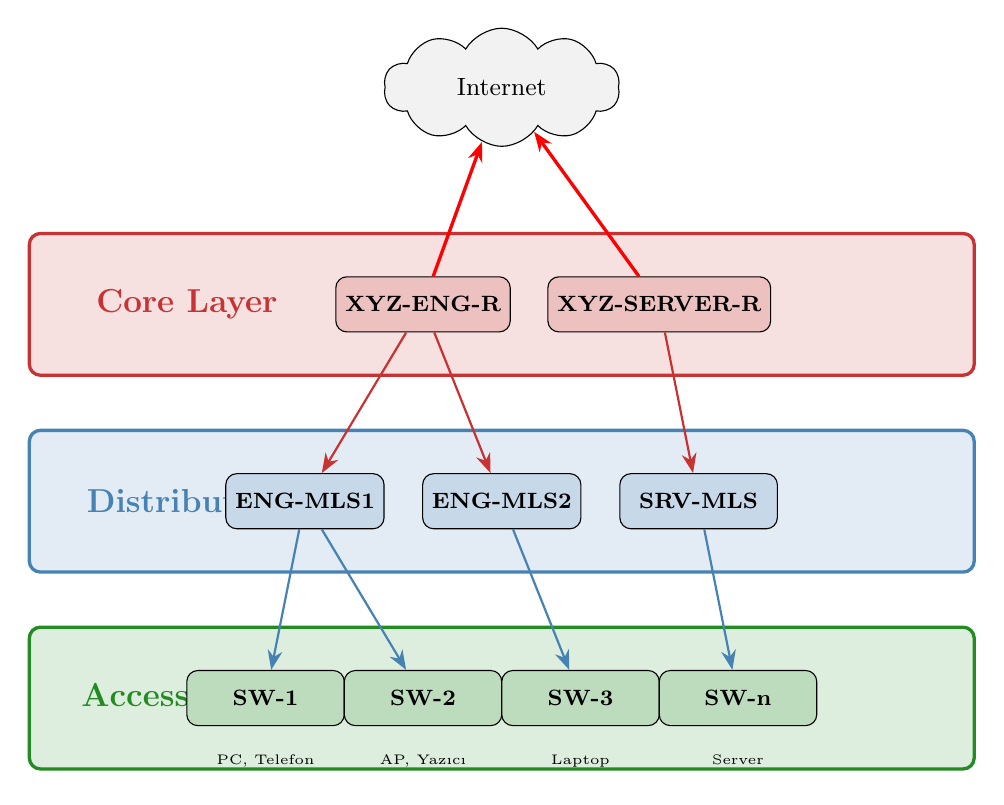
\begin{tikzpicture}[
  every node/.style={font=\small},
  layer/.style={draw, rounded corners, minimum width=12cm, minimum height=1.8cm, line width=1.2pt},
  device/.style={draw, rounded corners, minimum width=2cm, minimum height=0.7cm, font=\footnotesize\bfseries},
  conn/.style={-{Stealth[length=2.5mm]}, thick}
]

% Core Layer
\node[layer, fill=corered!15, draw=corered] (core) at (0,6) {};
\node[font=\bfseries\large, color=corered] at (-4,6) {Core Layer};
\node[device, fill=corered!30] (r1) at (-1,6) {XYZ-ENG-R};
\node[device, fill=corered!30] (r2) at (2,6) {XYZ-SERVER-R};

% Distribution Layer
\node[layer, fill=distblue!15, draw=distblue] (dist) at (0,3.5) {};
\node[font=\bfseries\large, color=distblue] at (-4,3.5) {Distribution};
\node[device, fill=distblue!30] (m1) at (-2.5,3.5) {ENG-MLS1};
\node[device, fill=distblue!30] (m2) at (0,3.5) {ENG-MLS2};
\node[device, fill=distblue!30] (m3) at (2.5,3.5) {SRV-MLS};

% Access Layer
\node[layer, fill=accessgreen!15, draw=accessgreen] (acc) at (0,1) {};
\node[font=\bfseries\large, color=accessgreen] at (-4,1) {Access Layer};
\node[device, fill=accessgreen!30] (s1) at (-3,1) {SW-1};
\node[device, fill=accessgreen!30] (s2) at (-1,1) {SW-2};
\node[device, fill=accessgreen!30] (s3) at (1,1) {SW-3};
\node[device, fill=accessgreen!30] (s4) at (3,1) {SW-n};

% Connections
\draw[conn, corered] (r1) -- (m1);
\draw[conn, corered] (r1) -- (m2);
\draw[conn, corered] (r2) -- (m3);
\draw[conn, distblue] (m1) -- (s1);
\draw[conn, distblue] (m1) -- (s2);
\draw[conn, distblue] (m2) -- (s3);
\draw[conn, distblue] (m3) -- (s4);

% Internet
\node[draw, cloud, cloud puffs=10, cloud puff arc=120, aspect=2,
      minimum width=3cm, minimum height=1.5cm, fill=gray!10,
      above=0.5cm of core] (inet) at (0,7.5) {Internet};
\draw[conn, red, very thick] (r1) -- (inet);
\draw[conn, red, very thick] (r2) -- (inet);

% Labels
\node[font=\tiny, below=0.1cm] at (-3,0.5) {PC, Telefon};
\node[font=\tiny, below=0.1cm] at (-1,0.5) {AP, Yazıcı};
\node[font=\tiny, below=0.1cm] at (1,0.5) {Laptop};
\node[font=\tiny, below=0.1cm] at (3,0.5) {Server};

\end{tikzpicture}
\caption{Üç Katmanlı Hiyerarşik Ağ Modeli}
\label{fig:three-layer}
\end{figure}

\begin{itemize}
  \item \textbf{\textcolor{corered}{Core Layer:}} Tüm yönlendiricilerin ve ana switch'lerin birbirine en yüksek hızda bağlandığı, ağın omurgasını oluşturan katmandır.
  \item \textbf{\textcolor{distblue}{Distribution Layer:}} Her fakülte veya birimin VLAN trafiğini core'a ileten ve erişim katmanına servis sağlayan yapıdadır.
  \item \textbf{\textcolor{accessgreen}{Access Layer:}} Son kullanıcıların, laboratuvarların ve ofis cihazlarının ağa bağlandığı katmandır.
\end{itemize}

\subsection{Proje Topolojisi (Cisco Packet Tracer)}

\begin{figure}[H]
  \centering
  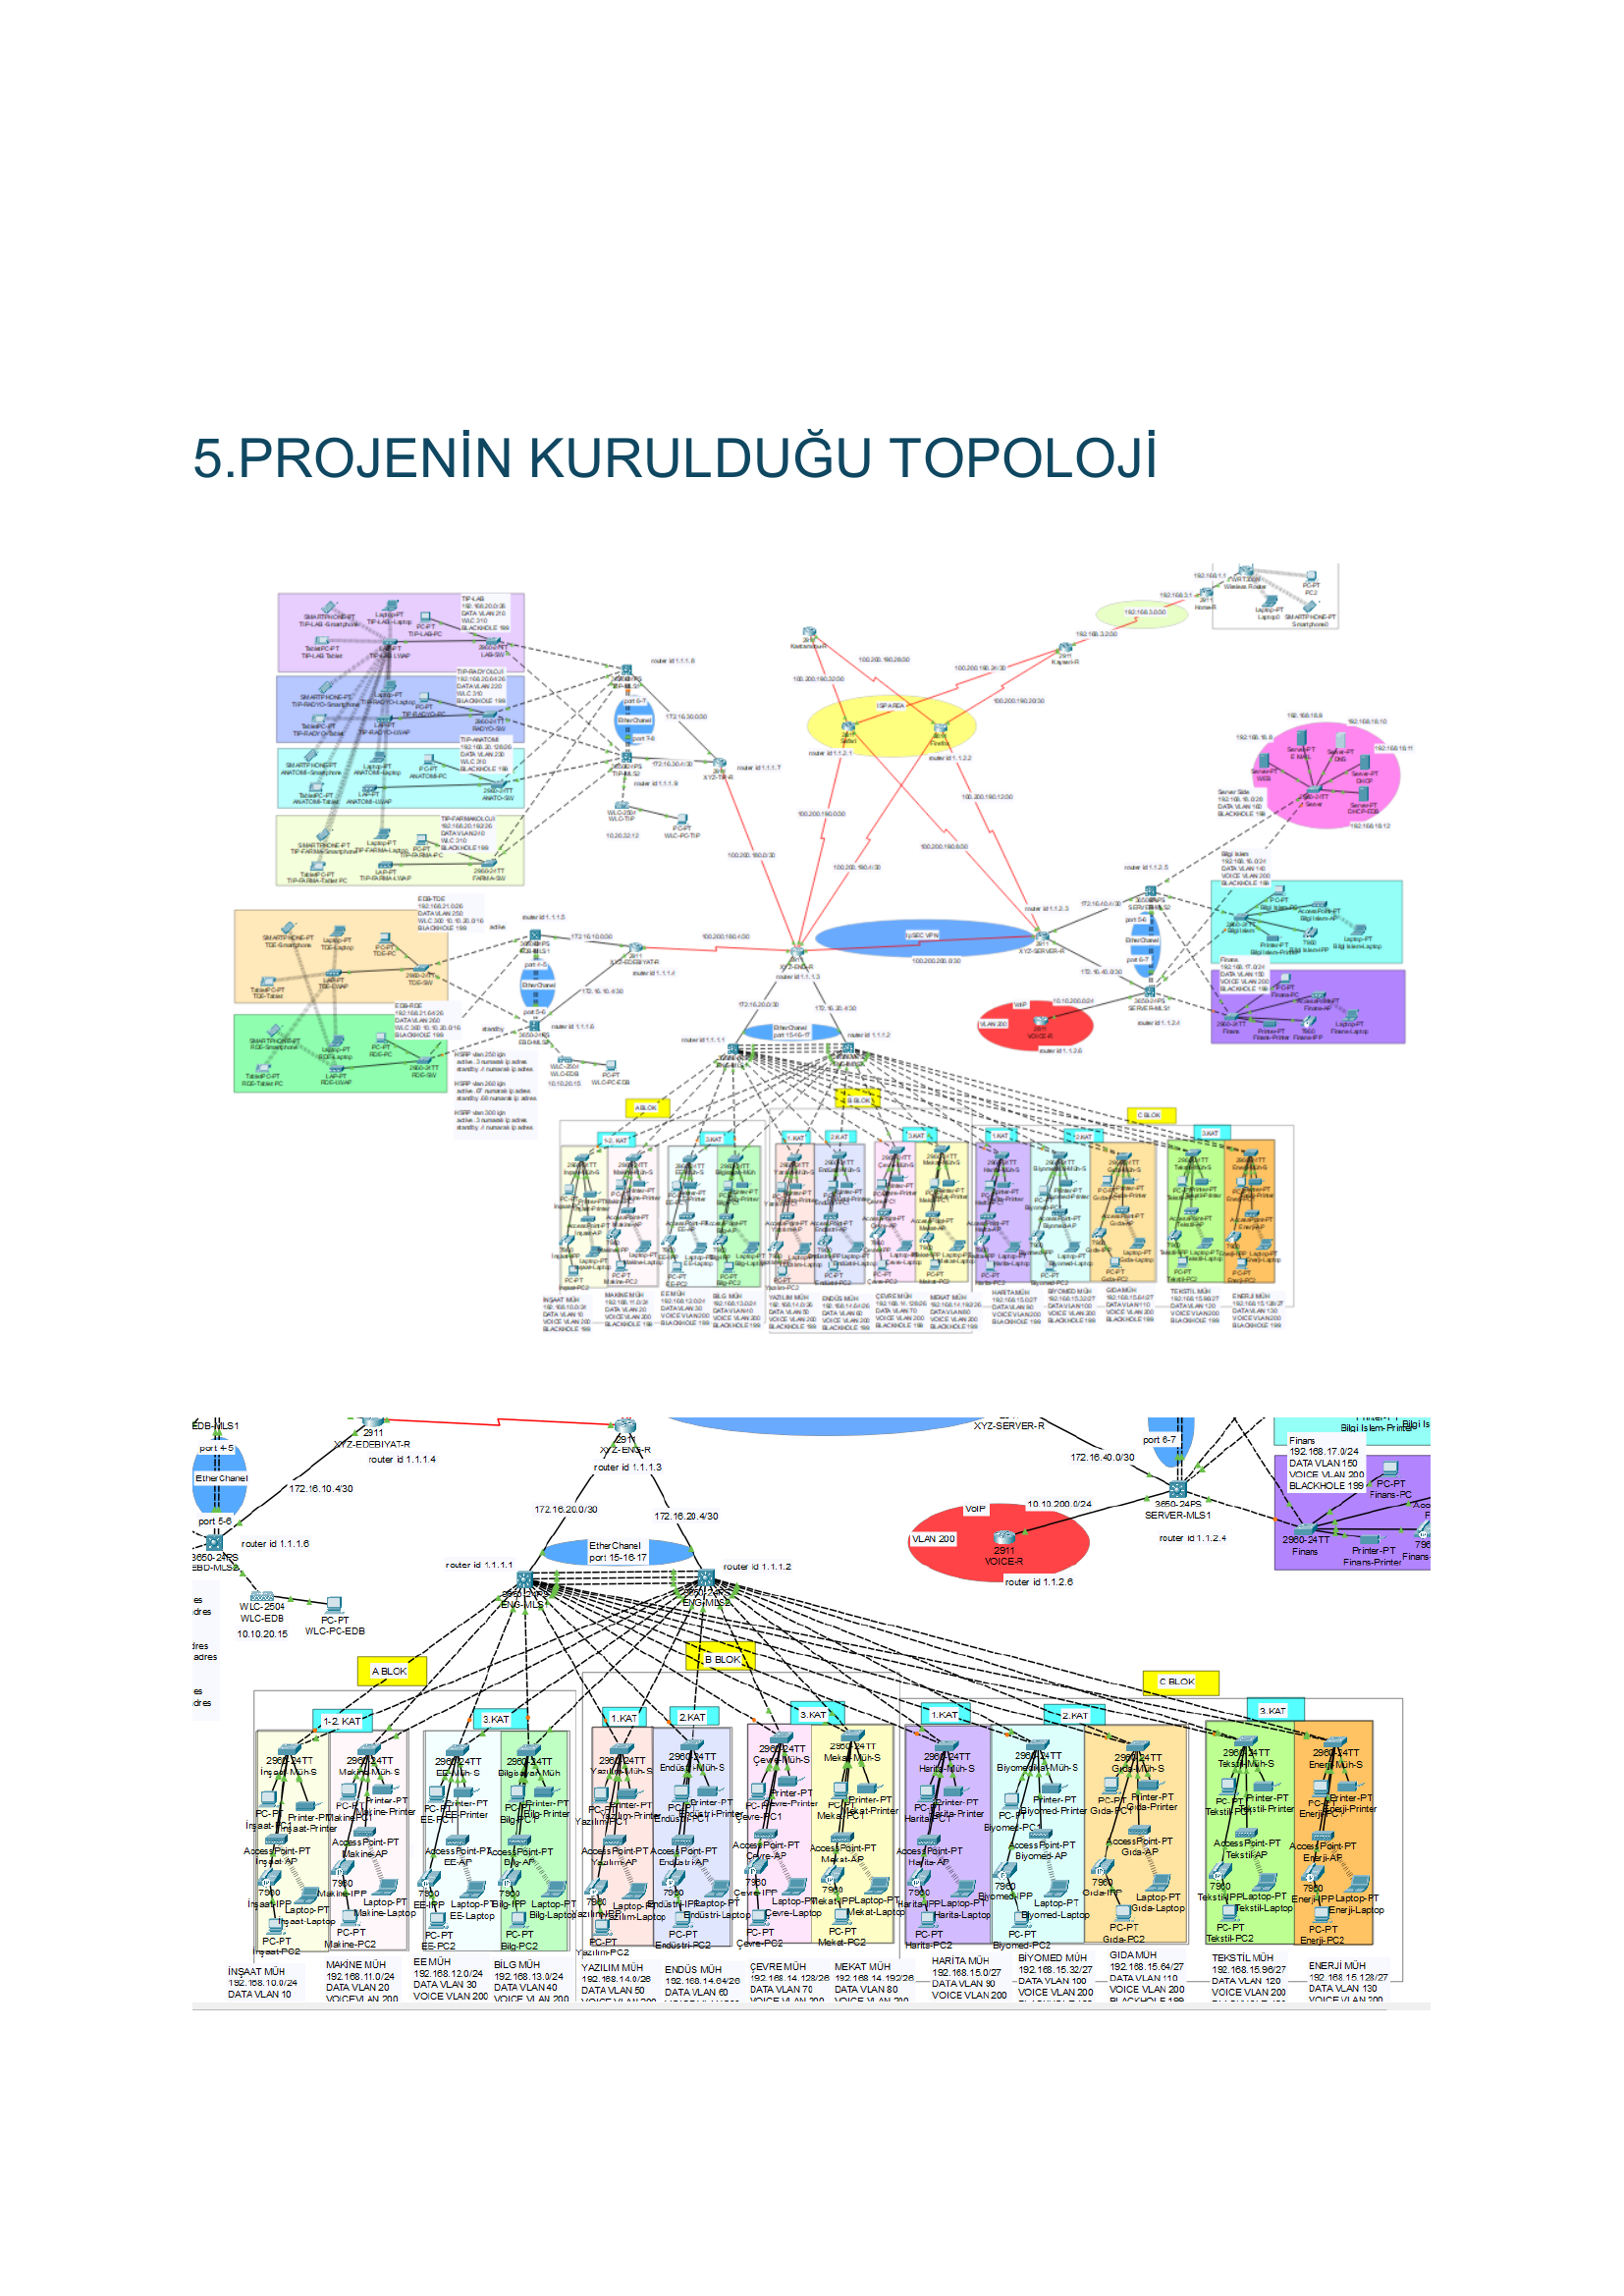
\includegraphics[width=\textwidth]{figures/topology-overview-1.png}
  \caption{Kampüs Ağı Genel Topolojisi -- Bölüm 1}
  \label{fig:topology1}
\end{figure}

\begin{figure}[H]
  \centering
  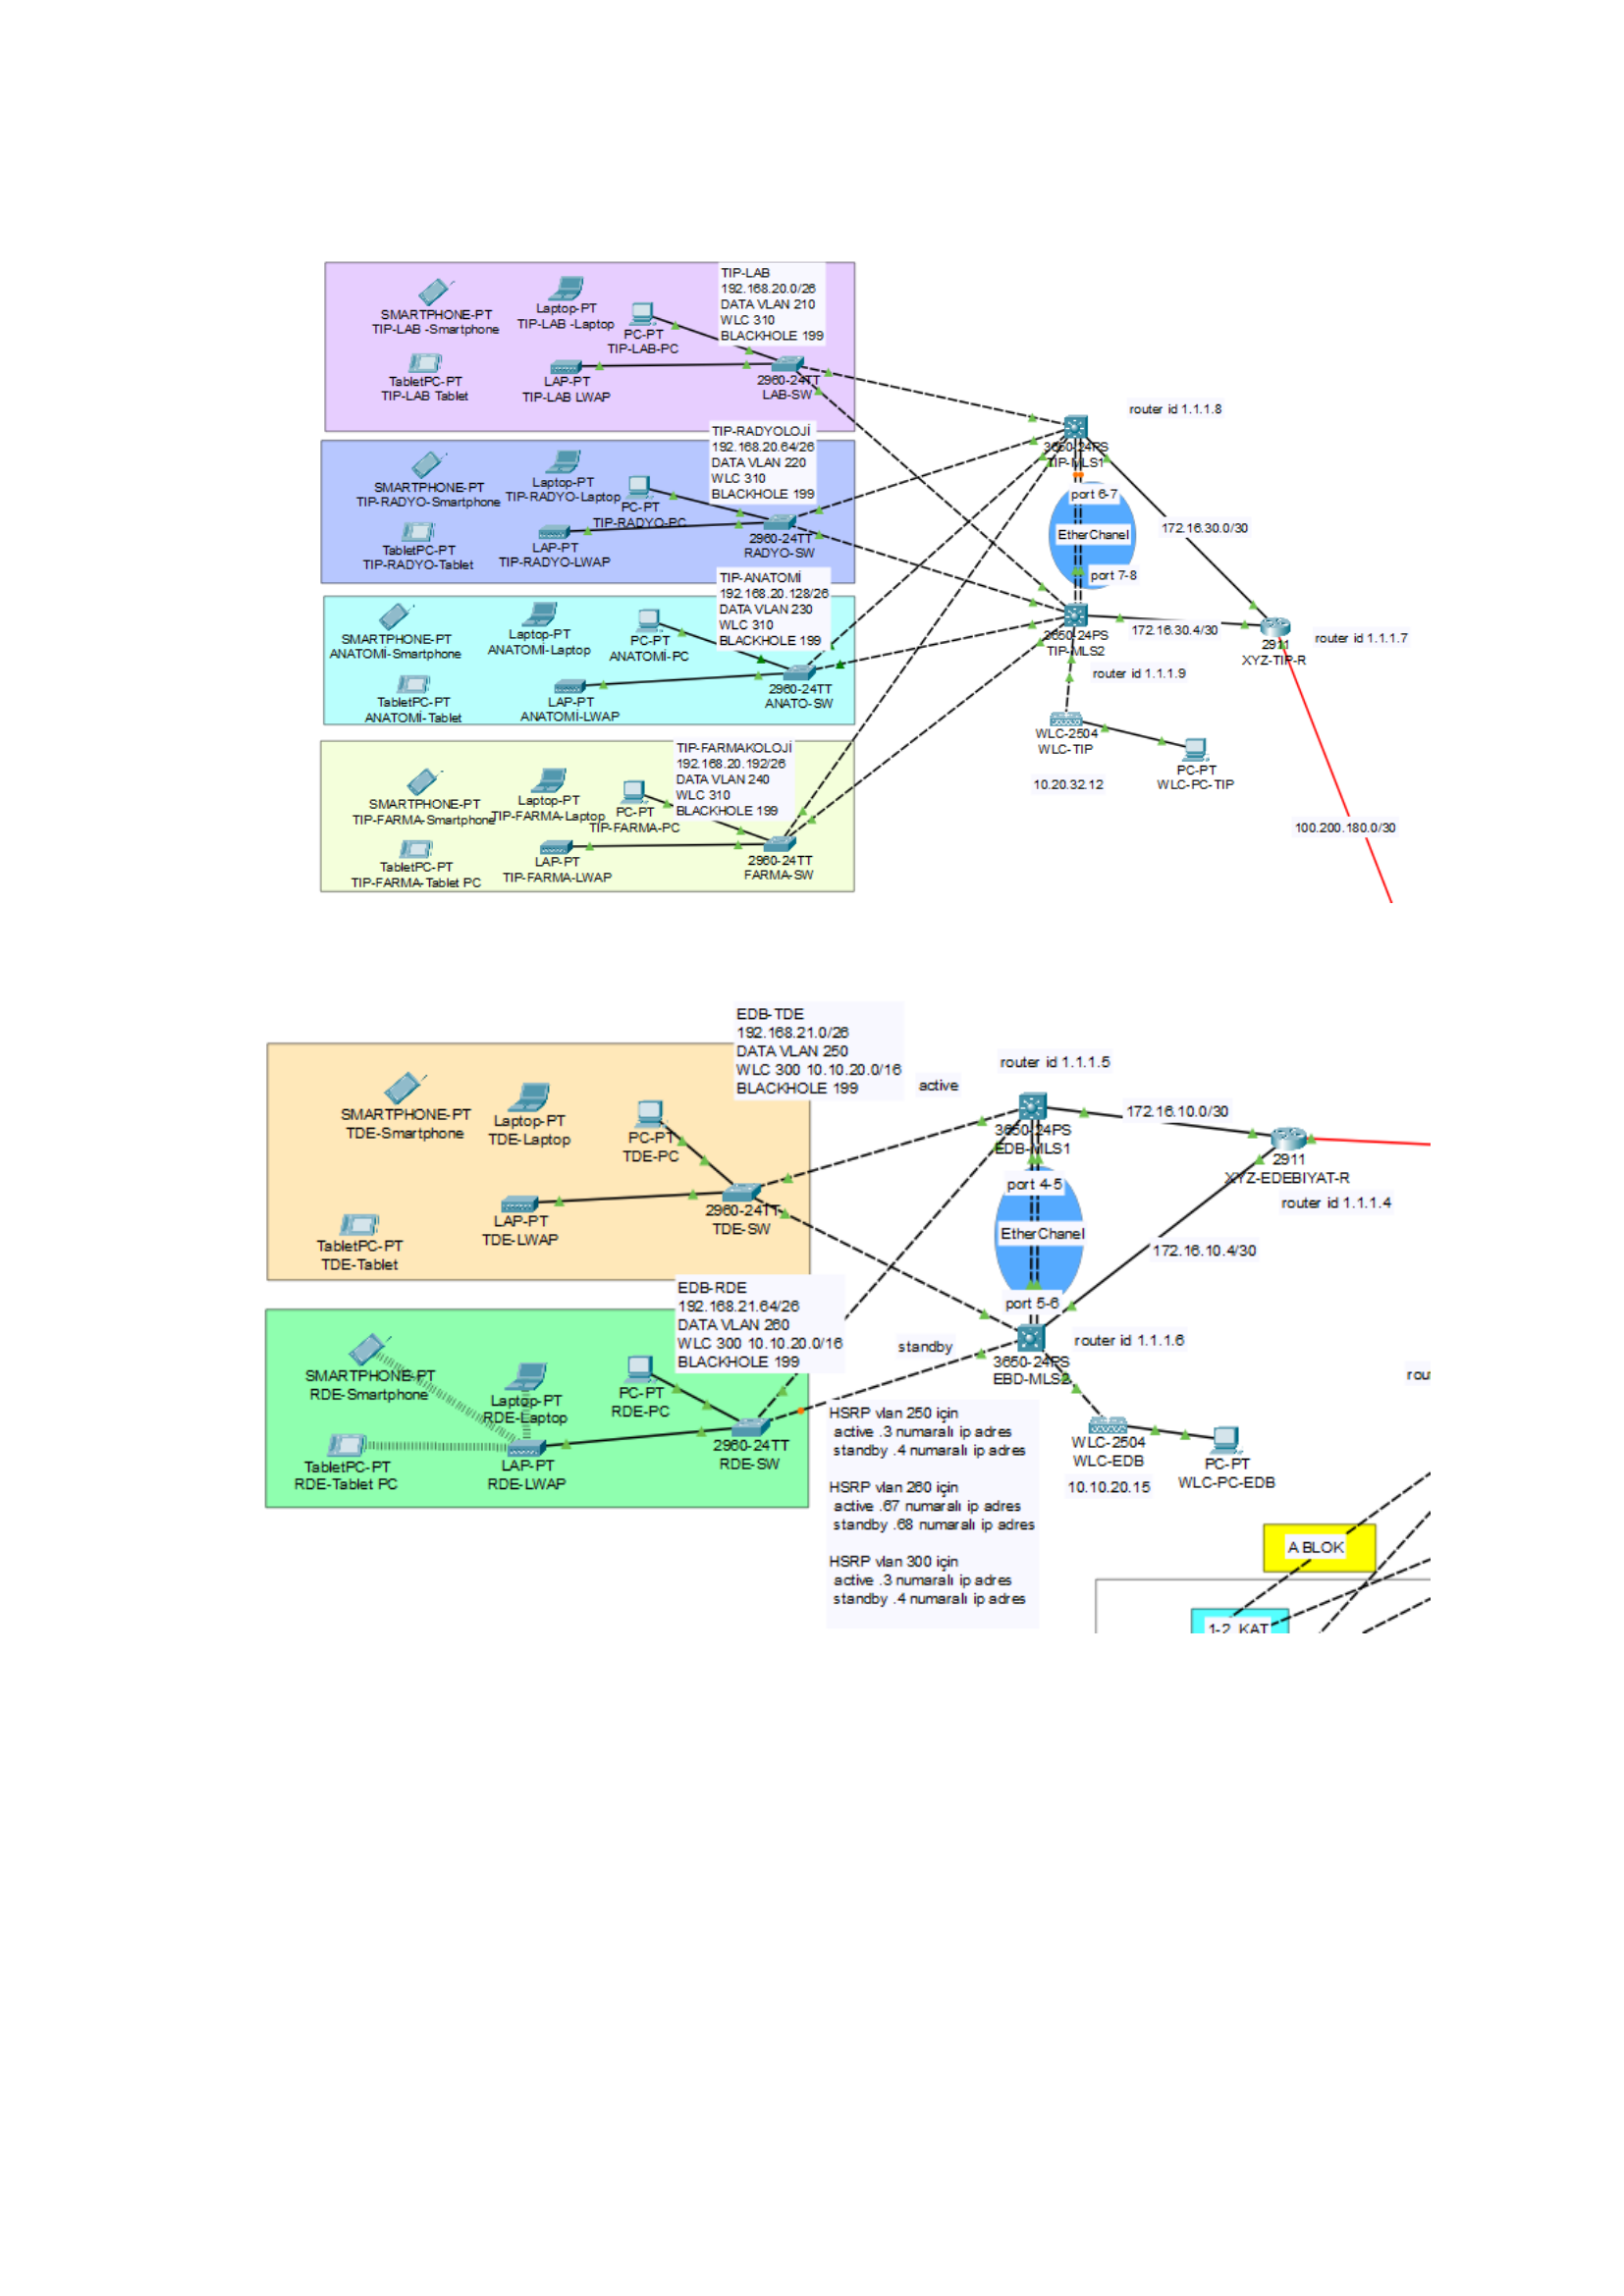
\includegraphics[width=\textwidth]{figures/topology-overview-2.png}
  \caption{Kampüs Ağı Genel Topolojisi -- Bölüm 2}
  \label{fig:topology2}
\end{figure}

% =========================================
% 3. VLAN YAPISI
% =========================================
\newpage
\section{VLAN Yapısı ve Ağ Segmentasyonu}

Kampüs içindeki her fakülte ve her idari birim için ayrı bir VLAN belirlenmiştir. Her VLAN kendi IP aralığı ile tanımlanmış ve DHCP tarafından yönetilmektedir.

% --- TikZ: VLAN Segmentation Diagram ---
\begin{figure}[H]
\centering
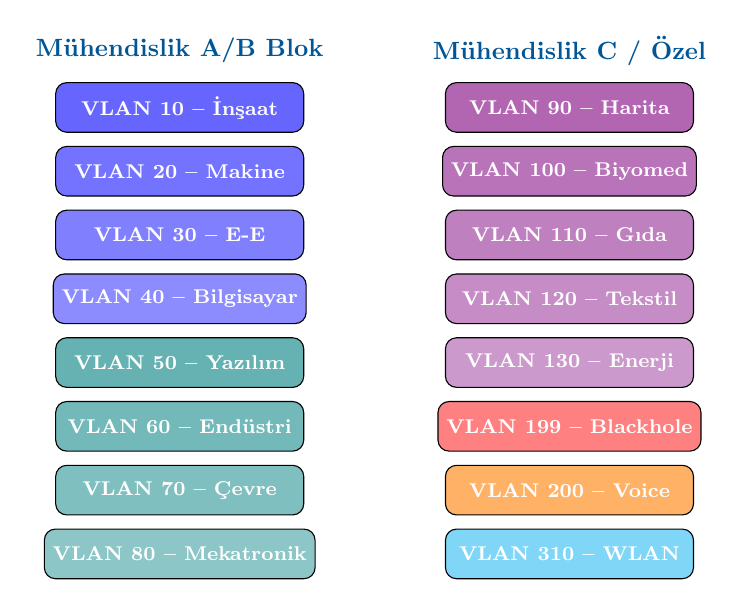
\begin{tikzpicture}[
  vlanbox/.style={draw, rounded corners, minimum width=3.5cm, minimum height=0.7cm, font=\footnotesize\bfseries, text=white},
  scale=0.9, transform shape
]

% VLAN boxes
\node[vlanbox, fill=blue!60] (v10) at (0,0) {VLAN 10 -- İnşaat};
\node[vlanbox, fill=blue!55] (v20) at (0,-0.9) {VLAN 20 -- Makine};
\node[vlanbox, fill=blue!50] (v30) at (0,-1.8) {VLAN 30 -- E-E};
\node[vlanbox, fill=blue!45] (v40) at (0,-2.7) {VLAN 40 -- Bilgisayar};
\node[vlanbox, fill=teal!60] (v50) at (0,-3.6) {VLAN 50 -- Yazılım};
\node[vlanbox, fill=teal!55] (v60) at (0,-4.5) {VLAN 60 -- Endüstri};
\node[vlanbox, fill=teal!50] (v70) at (0,-5.4) {VLAN 70 -- Çevre};
\node[vlanbox, fill=teal!45] (v80) at (0,-6.3) {VLAN 80 -- Mekatronik};

\node[vlanbox, fill=violet!60] (v90) at (5.5,0) {VLAN 90 -- Harita};
\node[vlanbox, fill=violet!55] (v100) at (5.5,-0.9) {VLAN 100 -- Biyomed};
\node[vlanbox, fill=violet!50] (v110) at (5.5,-1.8) {VLAN 110 -- Gıda};
\node[vlanbox, fill=violet!45] (v120) at (5.5,-2.7) {VLAN 120 -- Tekstil};
\node[vlanbox, fill=violet!40] (v130) at (5.5,-3.6) {VLAN 130 -- Enerji};

\node[vlanbox, fill=red!50] (v199) at (5.5,-4.5) {VLAN 199 -- Blackhole};
\node[vlanbox, fill=orange!60] (v200) at (5.5,-5.4) {VLAN 200 -- Voice};
\node[vlanbox, fill=cyan!50] (v310) at (5.5,-6.3) {VLAN 310 -- WLAN};

% Labels
\node[font=\bfseries, color=ciscoblue] at (0,0.8) {Mühendislik A/B Blok};
\node[font=\bfseries, color=ciscoblue] at (5.5,0.8) {Mühendislik C / Özel};

\end{tikzpicture}
\caption{VLAN Segmentasyonu}
\label{fig:vlan}
\end{figure}

% =========================================
% 4. IP SUBNETTING
% =========================================
\newpage
\section{IP Adresleme ve Subnetting}

\subsection{Mühendislik Fakültesi}

\begin{longtable}{lllll}
\toprule
\textbf{Bölüm} & \textbf{Network/Mask} & \textbf{Host Aralığı} & \textbf{Gateway} & \textbf{Broadcast} \\
\midrule
\endhead
İnşaat Müh. & 192.168.10.0/24 & .1 -- .254 & .1 & .255 \\
Makine Müh. & 192.168.11.0/24 & .1 -- .254 & .1 & .255 \\
E-E Müh. & 192.168.12.0/24 & .1 -- .254 & .1 & .255 \\
Bilgisayar Müh. & 192.168.13.0/24 & .1 -- .254 & .1 & .255 \\
Yazılım Müh. & 192.168.14.0/26 & .1 -- .62 & .1 & .63 \\
Endüstri Müh. & 192.168.14.64/26 & .65 -- .126 & .65 & .127 \\
Çevre Müh. & 192.168.14.128/26 & .129 -- .190 & .129 & .191 \\
Mekatronik Müh. & 192.168.14.192/26 & .193 -- .254 & .193 & .255 \\
Harita Müh. & 192.168.15.0/27 & .1 -- .30 & .1 & .31 \\
Biyomed Müh. & 192.168.15.32/27 & .33 -- .62 & .33 & .63 \\
Gıda Müh. & 192.168.15.64/27 & .65 -- .94 & .65 & .95 \\
Tekstil Müh. & 192.168.15.96/27 & .97 -- .126 & .97 & .127 \\
Enerji Müh. & 192.168.15.128/27 & .129 -- .158 & .129 & .159 \\
\bottomrule
\end{longtable}

\subsection{Server ve İdari Birimler}

\begin{longtable}{lllll}
\toprule
\textbf{Bölüm} & \textbf{Network/Mask} & \textbf{Host Aralığı} & \textbf{Gateway} & \textbf{Broadcast} \\
\midrule
\endhead
Bilgi İşlem & 192.168.16.0/24 & .1 -- .254 & .1 & .255 \\
Finans & 192.168.17.0/24 & .1 -- .254 & .1 & .255 \\
Server Room & 192.168.18.0/28 & .1 -- .14 & .1 & .15 \\
\bottomrule
\end{longtable}

\subsection{Tıp Fakültesi}

\begin{longtable}{lllll}
\toprule
\textbf{Bölüm} & \textbf{Network/Mask} & \textbf{Host Aralığı} & \textbf{Gateway} & \textbf{Broadcast} \\
\midrule
\endhead
Tıp-LAB & 192.168.20.0/26 & .1 -- .62 & .1 & .63 \\
Tıp-Radyoloji & 192.168.20.64/26 & .65 -- .126 & .65 & .127 \\
Tıp-Anatomi & 192.168.20.128/26 & .129 -- .190 & .129 & .191 \\
Tıp-Farmakoloji & 192.168.20.192/26 & .193 -- .254 & .193 & .255 \\
\bottomrule
\end{longtable}

\subsection{Edebiyat Fakültesi}

\begin{longtable}{lllll}
\toprule
\textbf{Bölüm} & \textbf{Network/Mask} & \textbf{Host Aralığı} & \textbf{Gateway} & \textbf{Broadcast} \\
\midrule
\endhead
EDB-TDE & 192.168.21.0/26 & .1 -- .62 & .1 & .63 \\
EDB-RDE & 192.168.21.64/26 & .65 -- .126 & .65 & .127 \\
\bottomrule
\end{longtable}

\subsection{Router Bağlantıları}

\begin{longtable}{llll}
\toprule
\textbf{Kaynak $\rightarrow$ Hedef} & \textbf{Network/Mask} & \textbf{IP Aralığı} \\
\midrule
\endhead
XYZ-ENG-R $\rightarrow$ ENG-MLS1 & 172.16.20.0/30 & .1 -- .2 \\
XYZ-ENG-R $\rightarrow$ ENG-MLS2 & 172.16.20.4/30 & .5 -- .6 \\
XYZ-ENG-R $\rightarrow$ Safari & 100.200.190.0/30 & .1 -- .2 \\
XYZ-ENG-R $\rightarrow$ Firefox & 100.200.190.4/30 & .5 -- .6 \\
XYZ-ENG-R $\rightarrow$ XYZ-EDB-R & 100.200.180.4/30 & .5 -- .6 \\
XYZ-ENG-R $\rightarrow$ XYZ-TIP-R & 100.200.180.0/30 & .1 -- .2 \\
XYZ-SERVER-R $\rightarrow$ Safari & 100.200.190.8/30 & .9 -- .10 \\
XYZ-SERVER-R $\rightarrow$ Firefox & 100.200.190.12/30 & .13 -- .14 \\
XYZ-SERVER-R $\rightarrow$ SERVER-MLS1 & 172.16.40.0/30 & .1 -- .2 \\
XYZ-SERVER-R $\rightarrow$ SERVER-MLS2 & 172.16.40.4/30 & .5 -- .6 \\
XYZ-SERVER-R $\rightarrow$ VOICE-R & 10.10.200.0/24 & .1 -- .254 \\
XYZ-EDB-R $\rightarrow$ EDB-MLS1 & 172.16.10.0/30 & .1 -- .2 \\
XYZ-EDB-R $\rightarrow$ EDB-MLS2 & 172.16.10.4/30 & .5 -- .6 \\
XYZ-TIP-R $\rightarrow$ TIP-MLS1 & 172.16.30.0/30 & .1 -- .2 \\
XYZ-TIP-R $\rightarrow$ TIP-MLS2 & 172.16.30.4/30 & .5 -- .6 \\
\bottomrule
\end{longtable}

% =========================================
% 5. YAPILANDIRMALAR
% =========================================
\newpage
\section{Cihaz Yapılandırmaları}

Tüm yapılandırma dosyaları \texttt{configs/} dizininde ayrı dosyalar halinde bulunmaktadır.

\subsection{Temel Cihaz Yapılandırması}

\begin{infobox}[Açıklama]
Her switch ve router için temel güvenlik ayarları: hostname, şifreleme, SSH erişimi ve ACL ile yalnızca Bilgi İşlem biriminin erişimine izin verilmektedir.
\end{infobox}

\lstinputlisting[style=cisco, caption={Temel Cihaz Yapılandırması (\texttt{configs/01-basic-device.ios})}]{../configs/01-basic-device.ios}

\subsection{STP PortFast + BPDU Guard}

\begin{warningbox}[Dikkat]
Bu konfigürasyon trunk veya başka switch bağlantısı olan portlarda \textbf{kullanılmamalıdır}. Yalnızca uç (edge) cihazların bağlandığı portlarda kullanılmalıdır: PC, IP telefon, printer, access point, WLC.
\end{warningbox}

\lstinputlisting[style=cisco, caption={STP PortFast + BPDU Guard (\texttt{configs/02-stp-bpduguard.ios})}]{../configs/02-stp-bpduguard.ios}

\subsection{VLAN ve Trunk Yapılandırması}

\lstinputlisting[style=cisco, caption={Access Layer -- VLAN ve Trunk (\texttt{configs/03-vlan-trunk-access.ios})}]{../configs/03-vlan-trunk-access.ios}

\subsection{Distribution Layer Yapılandırması}

\lstinputlisting[style=cisco, caption={Distribution Layer (\texttt{configs/04-distribution-layer.ios})}]{../configs/04-distribution-layer.ios}

\subsection{LACP -- EtherChannel}

% --- TikZ: EtherChannel Diagram ---
\begin{figure}[H]
\centering
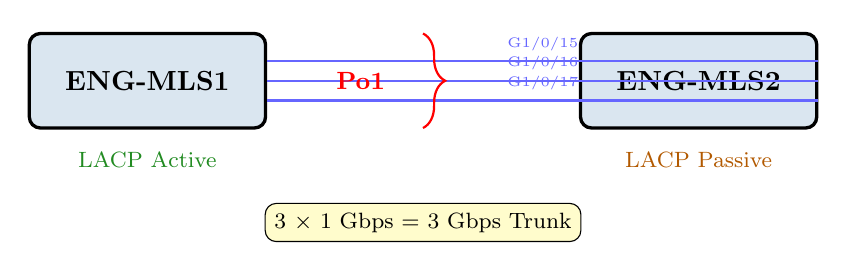
\begin{tikzpicture}[
  sw/.style={draw, rounded corners, minimum width=3cm, minimum height=1.2cm, fill=distblue!20, font=\bfseries, line width=1.2pt},
]
  \node[sw] (mls1) at (0,0) {ENG-MLS1};
  \node[sw] (mls2) at (7,0) {ENG-MLS2};

  % Physical links
  \draw[thick, blue!60] (mls1.east) ++(0,0.25) -- ++(7,0) node[midway, above, font=\tiny] {G1/0/15};
  \draw[thick, blue!60] (mls1.east) ++(0,0) -- ++(7,0) node[midway, above, font=\tiny] {G1/0/16};
  \draw[thick, blue!60] (mls1.east) ++(0,-0.25) -- ++(7,0) node[midway, above, font=\tiny] {G1/0/17};

  % EtherChannel label
  \draw[decorate, decoration={brace, amplitude=8pt, mirror}, thick, red]
    (3.5,-0.6) -- (3.5,0.6) node[midway, left=10pt, font=\small\bfseries, red] {Po1};

  \node[font=\footnotesize, color=accessgreen] at (0,-1) {LACP Active};
  \node[font=\footnotesize, color=orange!70!black] at (7,-1) {LACP Passive};

  % Label
  \node[draw, rounded corners, fill=yellow!20, font=\footnotesize] at (3.5,-1.8) {3 $\times$ 1 Gbps = 3 Gbps Trunk};
\end{tikzpicture}
\caption{LACP EtherChannel Topolojisi}
\label{fig:etherchannel}
\end{figure}

\lstinputlisting[style=cisco, caption={LACP EtherChannel (\texttt{configs/05-lacp-etherchannel.ios})}]{../configs/05-lacp-etherchannel.ios}

\subsection{Port Security}

\lstinputlisting[style=cisco, caption={Port Security (\texttt{configs/06-port-security.ios})}]{../configs/06-port-security.ios}

\subsection{VoIP Sub-Interface}

\lstinputlisting[style=cisco, caption={VoIP Sub-Interface (\texttt{configs/07-voip-subinterface.ios})}]{../configs/07-voip-subinterface.ios}

\subsection{HSRP Yapılandırması}

% --- TikZ: HSRP Diagram ---
\begin{figure}[H]
\centering
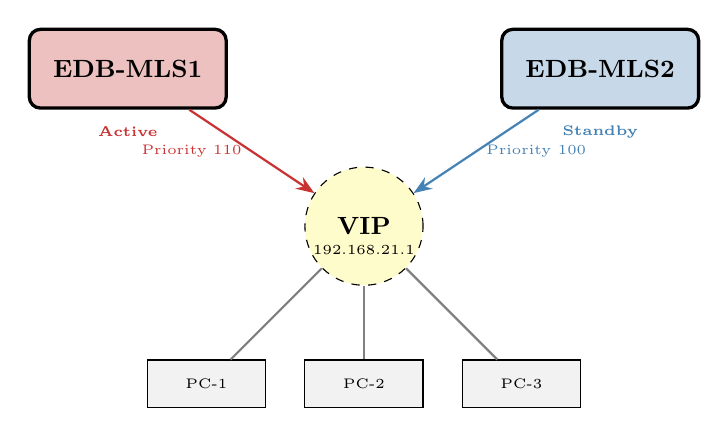
\begin{tikzpicture}[
  rtr/.style={draw, rounded corners, minimum width=2.5cm, minimum height=1cm, font=\small\bfseries, line width=1.2pt},
  pc/.style={draw, rectangle, minimum width=1.5cm, minimum height=0.6cm, fill=gray!10, font=\tiny},
]
  % Routers
  \node[rtr, fill=corered!30] (mls1) at (-2,2) {EDB-MLS1};
  \node[rtr, fill=distblue!30] (mls2) at (4,2) {EDB-MLS2};

  % Virtual IP
  \node[draw, dashed, circle, minimum size=1.5cm, fill=yellow!20, font=\small\bfseries] (vip) at (1,0) {VIP};

  % PCs
  \node[pc] (pc1) at (-1,-2) {PC-1};
  \node[pc] (pc2) at (1,-2) {PC-2};
  \node[pc] (pc3) at (3,-2) {PC-3};

  % Connections
  \draw[-{Stealth}, thick, corered] (mls1) -- (vip) node[midway, left, font=\tiny] {Priority 110};
  \draw[-{Stealth}, thick, distblue] (mls2) -- (vip) node[midway, right, font=\tiny] {Priority 100};
  \draw[thick, gray] (vip) -- (pc1);
  \draw[thick, gray] (vip) -- (pc2);
  \draw[thick, gray] (vip) -- (pc3);

  % Labels
  \node[font=\tiny\bfseries, color=corered] at (-2,1.2) {Active};
  \node[font=\tiny\bfseries, color=distblue] at (4,1.2) {Standby};
  \node[font=\tiny] at (1,-0.3) {192.168.21.1};
\end{tikzpicture}
\caption{HSRP Yedekli Gateway Yapısı}
\label{fig:hsrp}
\end{figure}

\lstinputlisting[style=cisco, caption={HSRP Yapılandırması (\texttt{configs/08-hsrp.ios})}]{../configs/08-hsrp.ios}

\subsection{DHCP Helper}

\lstinputlisting[style=cisco, caption={DHCP Helper (\texttt{configs/09-dhcp-helper.ios})}]{../configs/09-dhcp-helper.ios}

\subsection{OSPF Yapılandırması}

% --- TikZ: OSPF Topology ---
\begin{figure}[H]
\centering
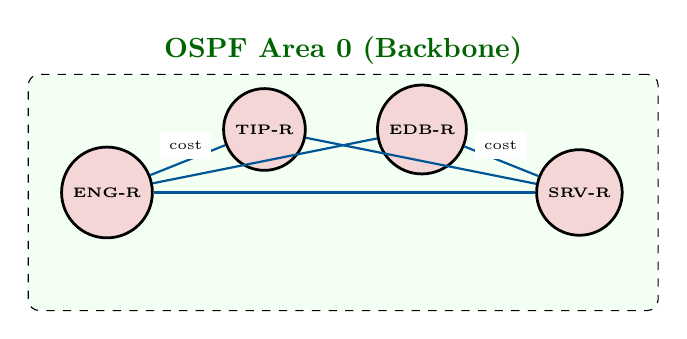
\begin{tikzpicture}[
  rtr/.style={draw, circle, minimum size=1cm, fill=corered!20, font=\tiny\bfseries, line width=1pt},
  area/.style={draw, dashed, rounded corners, minimum width=8cm, minimum height=3cm, fill=green!5},
]
  % Area 0
  \node[area] at (0,0) {};
  \node[font=\bfseries, color=darkgreen] at (0,1.8) {OSPF Area 0 (Backbone)};

  % Routers
  \node[rtr] (r1) at (-3,0) {ENG-R};
  \node[rtr] (r2) at (-1,0.8) {TIP-R};
  \node[rtr] (r3) at (1,0.8) {EDB-R};
  \node[rtr] (r4) at (3,0) {SRV-R};

  % Connections
  \draw[thick, ciscoblue] (r1) -- (r2);
  \draw[thick, ciscoblue] (r1) -- (r3);
  \draw[thick, ciscoblue] (r2) -- (r4);
  \draw[thick, ciscoblue] (r3) -- (r4);
  \draw[thick, ciscoblue] (r1) -- (r4);

  % Cost labels
  \node[font=\tiny, fill=white] at (-2,0.6) {cost};
  \node[font=\tiny, fill=white] at (2,0.6) {cost};

\end{tikzpicture}
\caption{OSPF Yönlendirme Topolojisi}
\label{fig:ospf}
\end{figure}

\lstinputlisting[style=cisco, caption={OSPF Yapılandırması (\texttt{configs/10-ospf.ios})}]{../configs/10-ospf.ios}

\subsection{VoIP ve Telephony Service}

\lstinputlisting[style=cisco, caption={VoIP / CME Yapılandırması (\texttt{configs/11-voip-telephony.ios})}]{../configs/11-voip-telephony.ios}

\subsection{NAT/PAT}

% --- TikZ: NAT/PAT Diagram ---
\begin{figure}[H]
\centering
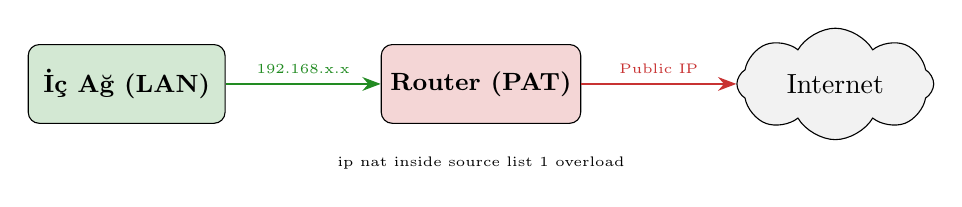
\begin{tikzpicture}[
  box/.style={draw, rounded corners, minimum width=2.5cm, minimum height=1cm, font=\small\bfseries},
]
  \node[box, fill=accessgreen!20] (lan) at (0,0) {İç Ağ (LAN)};
  \node[box, fill=corered!20] (rtr) at (4.5,0) {Router (PAT)};
  \node[draw, cloud, cloud puffs=8, cloud puff arc=120, aspect=2,
        minimum width=2.5cm, minimum height=1.2cm, fill=gray!10] (inet) at (9,0) {Internet};

  \draw[-{Stealth}, thick, accessgreen] (lan) -- (rtr) node[midway, above, font=\tiny] {192.168.x.x};
  \draw[-{Stealth}, thick, corered] (rtr) -- (inet) node[midway, above, font=\tiny] {Public IP};

  \node[font=\tiny, below=0.3cm of rtr] {ip nat inside source list 1 overload};
\end{tikzpicture}
\caption{NAT/PAT Yapısı}
\label{fig:natpat}
\end{figure}

\lstinputlisting[style=cisco, caption={NAT/PAT (\texttt{configs/12-nat-pat.ios})}]{../configs/12-nat-pat.ios}

\subsection{Site-to-Site IPsec VPN}

% --- TikZ: VPN Tunnel ---
\begin{figure}[H]
\centering
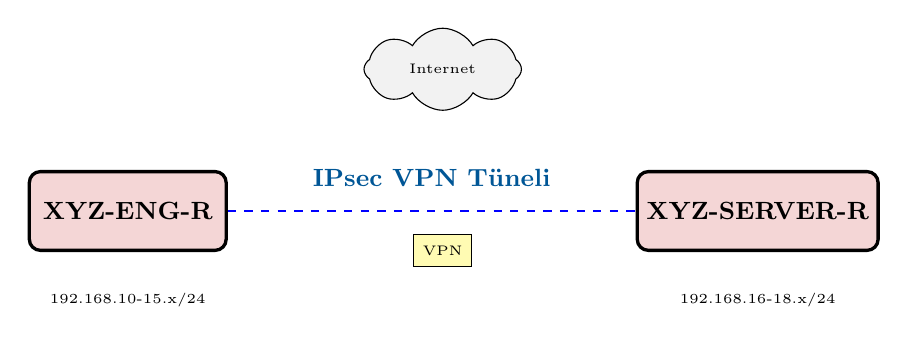
\begin{tikzpicture}[
  rtr/.style={draw, rounded corners, minimum width=2.5cm, minimum height=1cm, fill=corered!20, font=\small\bfseries, line width=1.2pt},
]
  \node[rtr] (eng) at (0,0) {XYZ-ENG-R};
  \node[rtr] (srv) at (8,0) {XYZ-SERVER-R};

  % Tunnel
  \draw[thick, blue, dashed]
    (eng.east) -- (srv.west) node[midway, above=5pt, font=\small\bfseries, color=ciscoblue] {IPsec VPN Tüneli};

  % Lock symbol
  \node[draw, fill=yellow!30, minimum size=0.4cm, font=\tiny] at (4,-0.5) {VPN};

  % Subnets
  \node[font=\tiny, below=0.4cm of eng] {192.168.10-15.x/24};
  \node[font=\tiny, below=0.4cm of srv] {192.168.16-18.x/24};

  % Internet
  \node[draw, cloud, cloud puffs=8, cloud puff arc=120, aspect=2,
        minimum width=2cm, minimum height=1cm, fill=gray!10] at (4,1.8) {\tiny Internet};
\end{tikzpicture}
\caption{Site-to-Site IPsec VPN Tüneli}
\label{fig:vpn}
\end{figure}

\lstinputlisting[style=cisco, caption={Site-to-Site VPN (\texttt{configs/13-vpn-ipsec.ios})}]{../configs/13-vpn-ipsec.ios}

% =========================================
% 6. TEST VE DOĞRULAMA
% =========================================
\newpage
\section{Test ve Doğrulama}

Ağ yapılandırmasının doğruluğunu teyit etmek için aşağıdaki testler gerçekleştirilmiştir.

\subsection{DHCP IP Ataması ve DNS Testi}

DHCP sunucusundan başarıyla IP adresi alınması ve \texttt{erü.öbs} alan adının DNS çözümlemesi doğrulanmıştır.

\begin{figure}[H]
  \centering
  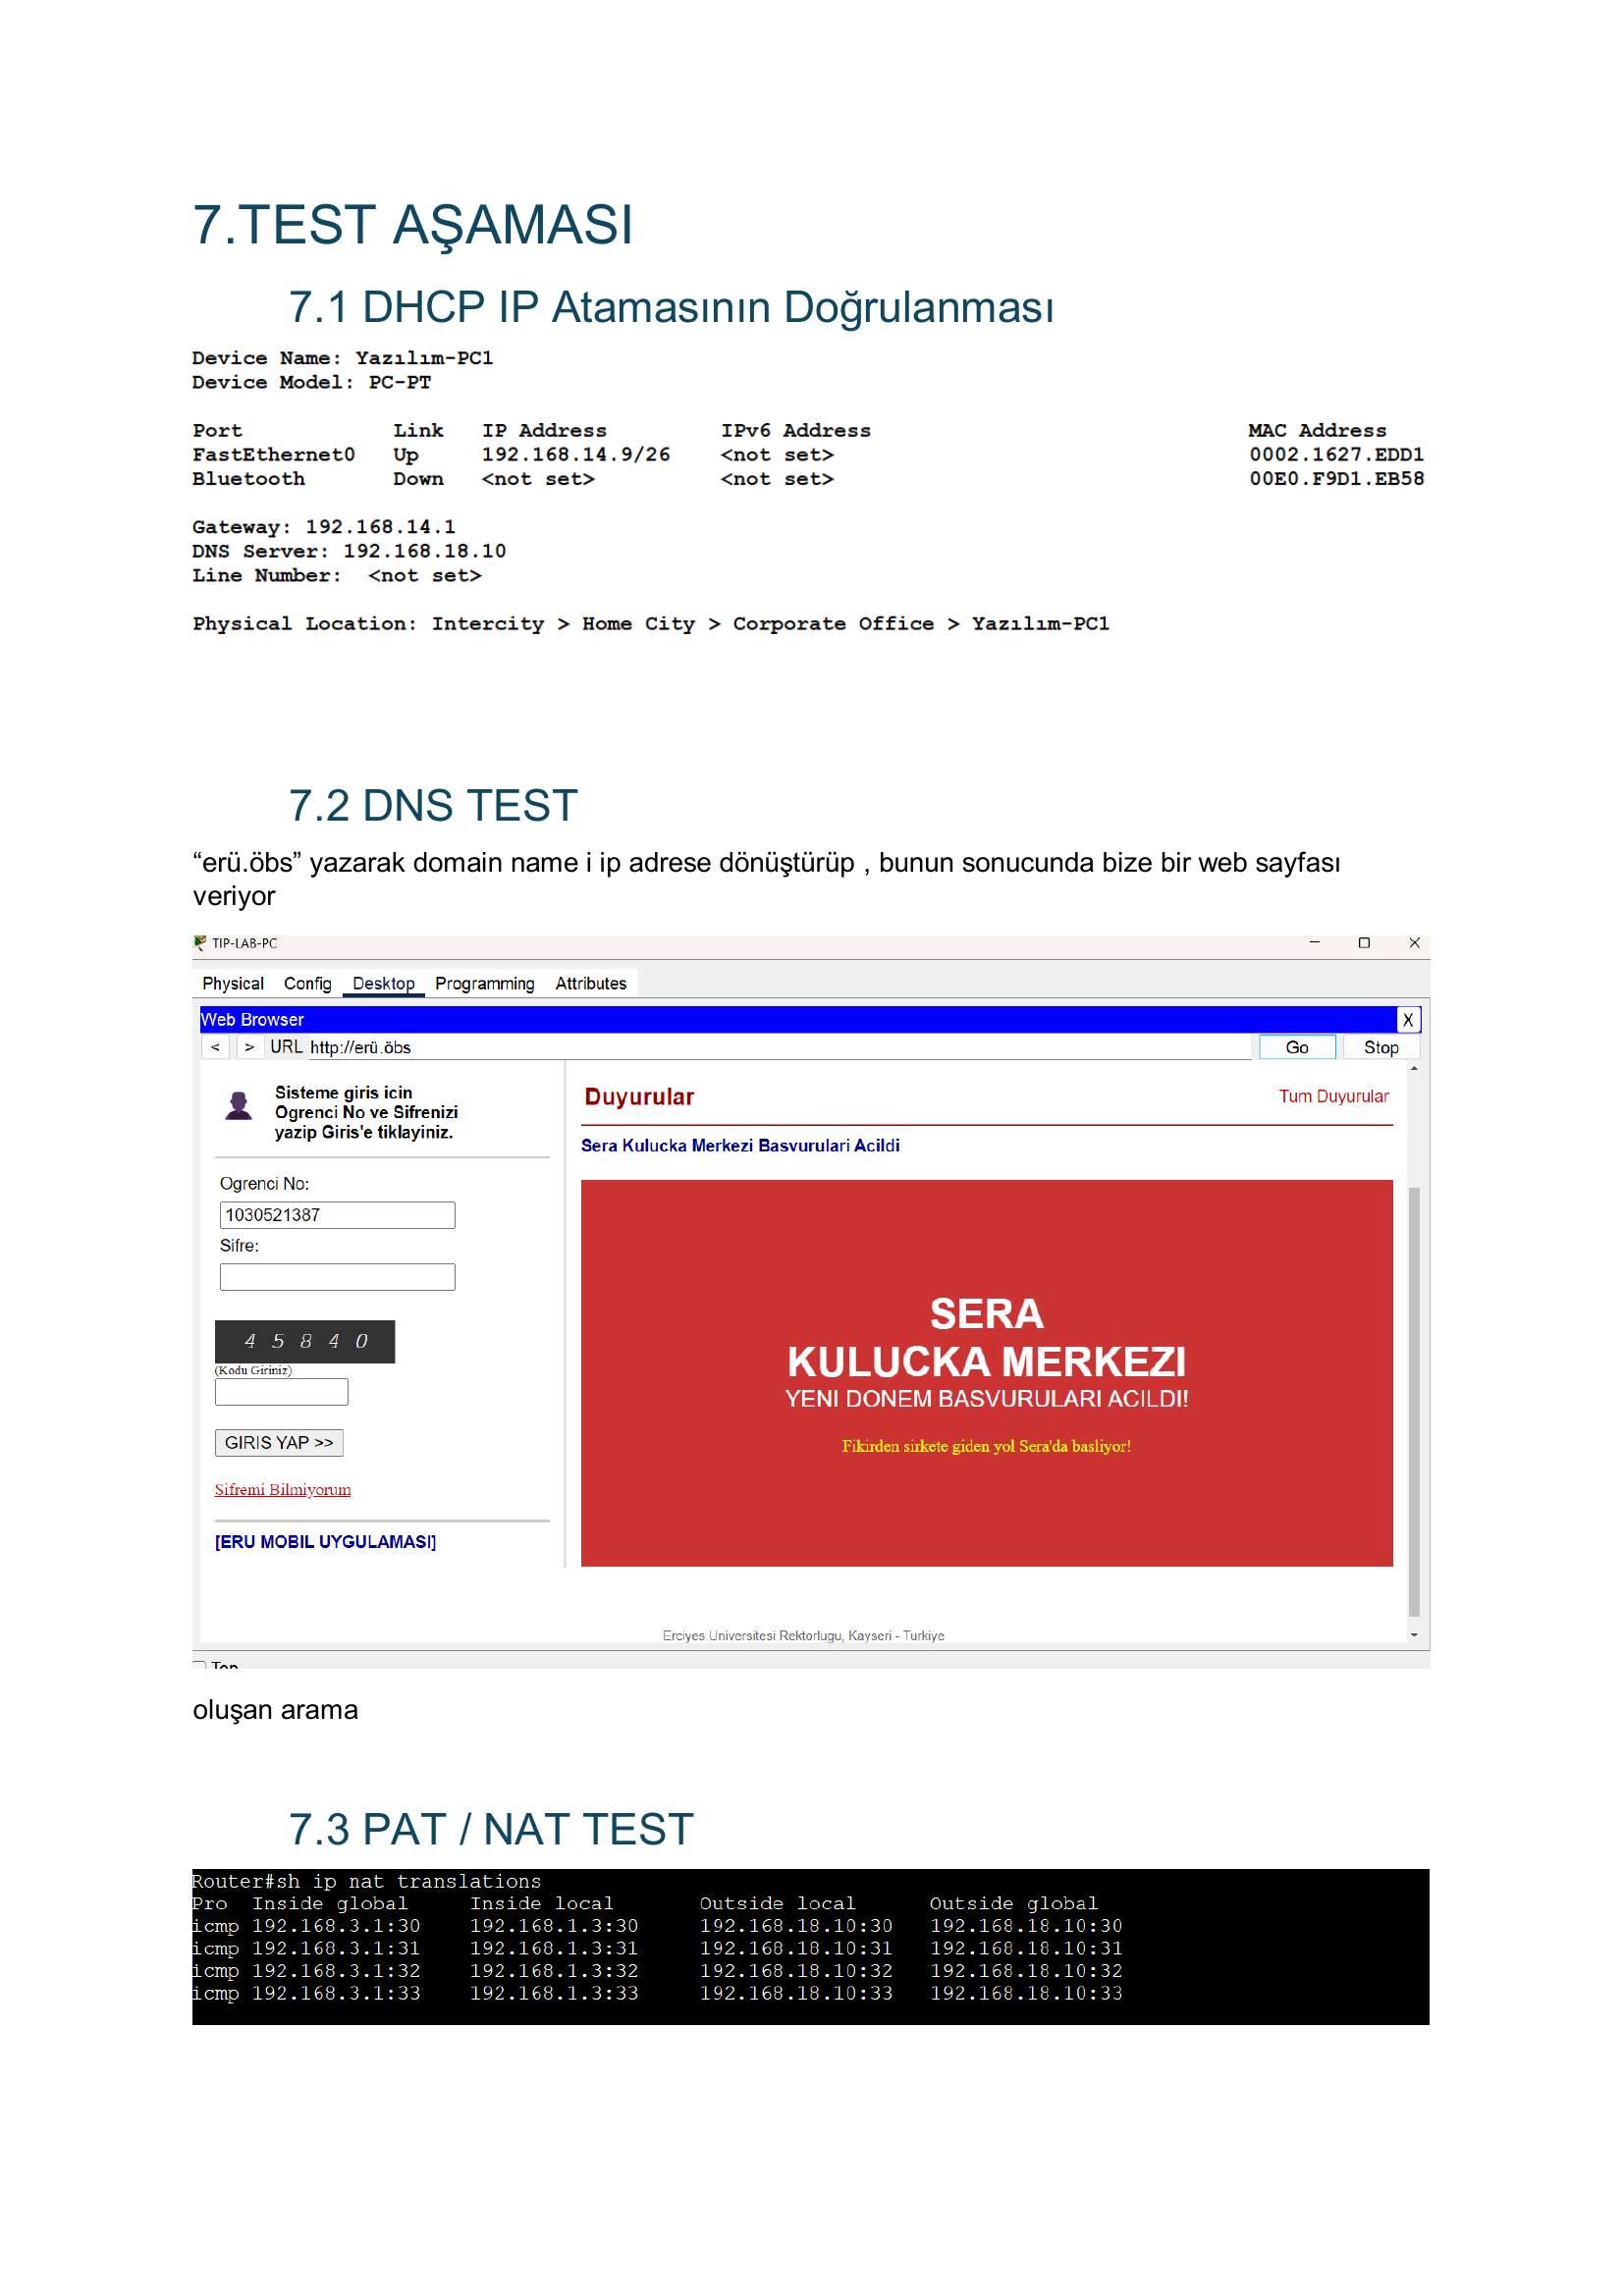
\includegraphics[width=0.85\textwidth]{figures/test-dhcp-dns.png}
  \caption{DHCP IP Ataması ve DNS Testi}
  \label{fig:test-dhcp}
\end{figure}

\subsection{PAT/NAT ve VPN Testi}

Dışarıdan WEB Server'a erişim (PAT) ve VPN öncesi/sonrası trace route karşılaştırması yapılmıştır.

\begin{figure}[H]
  \centering
  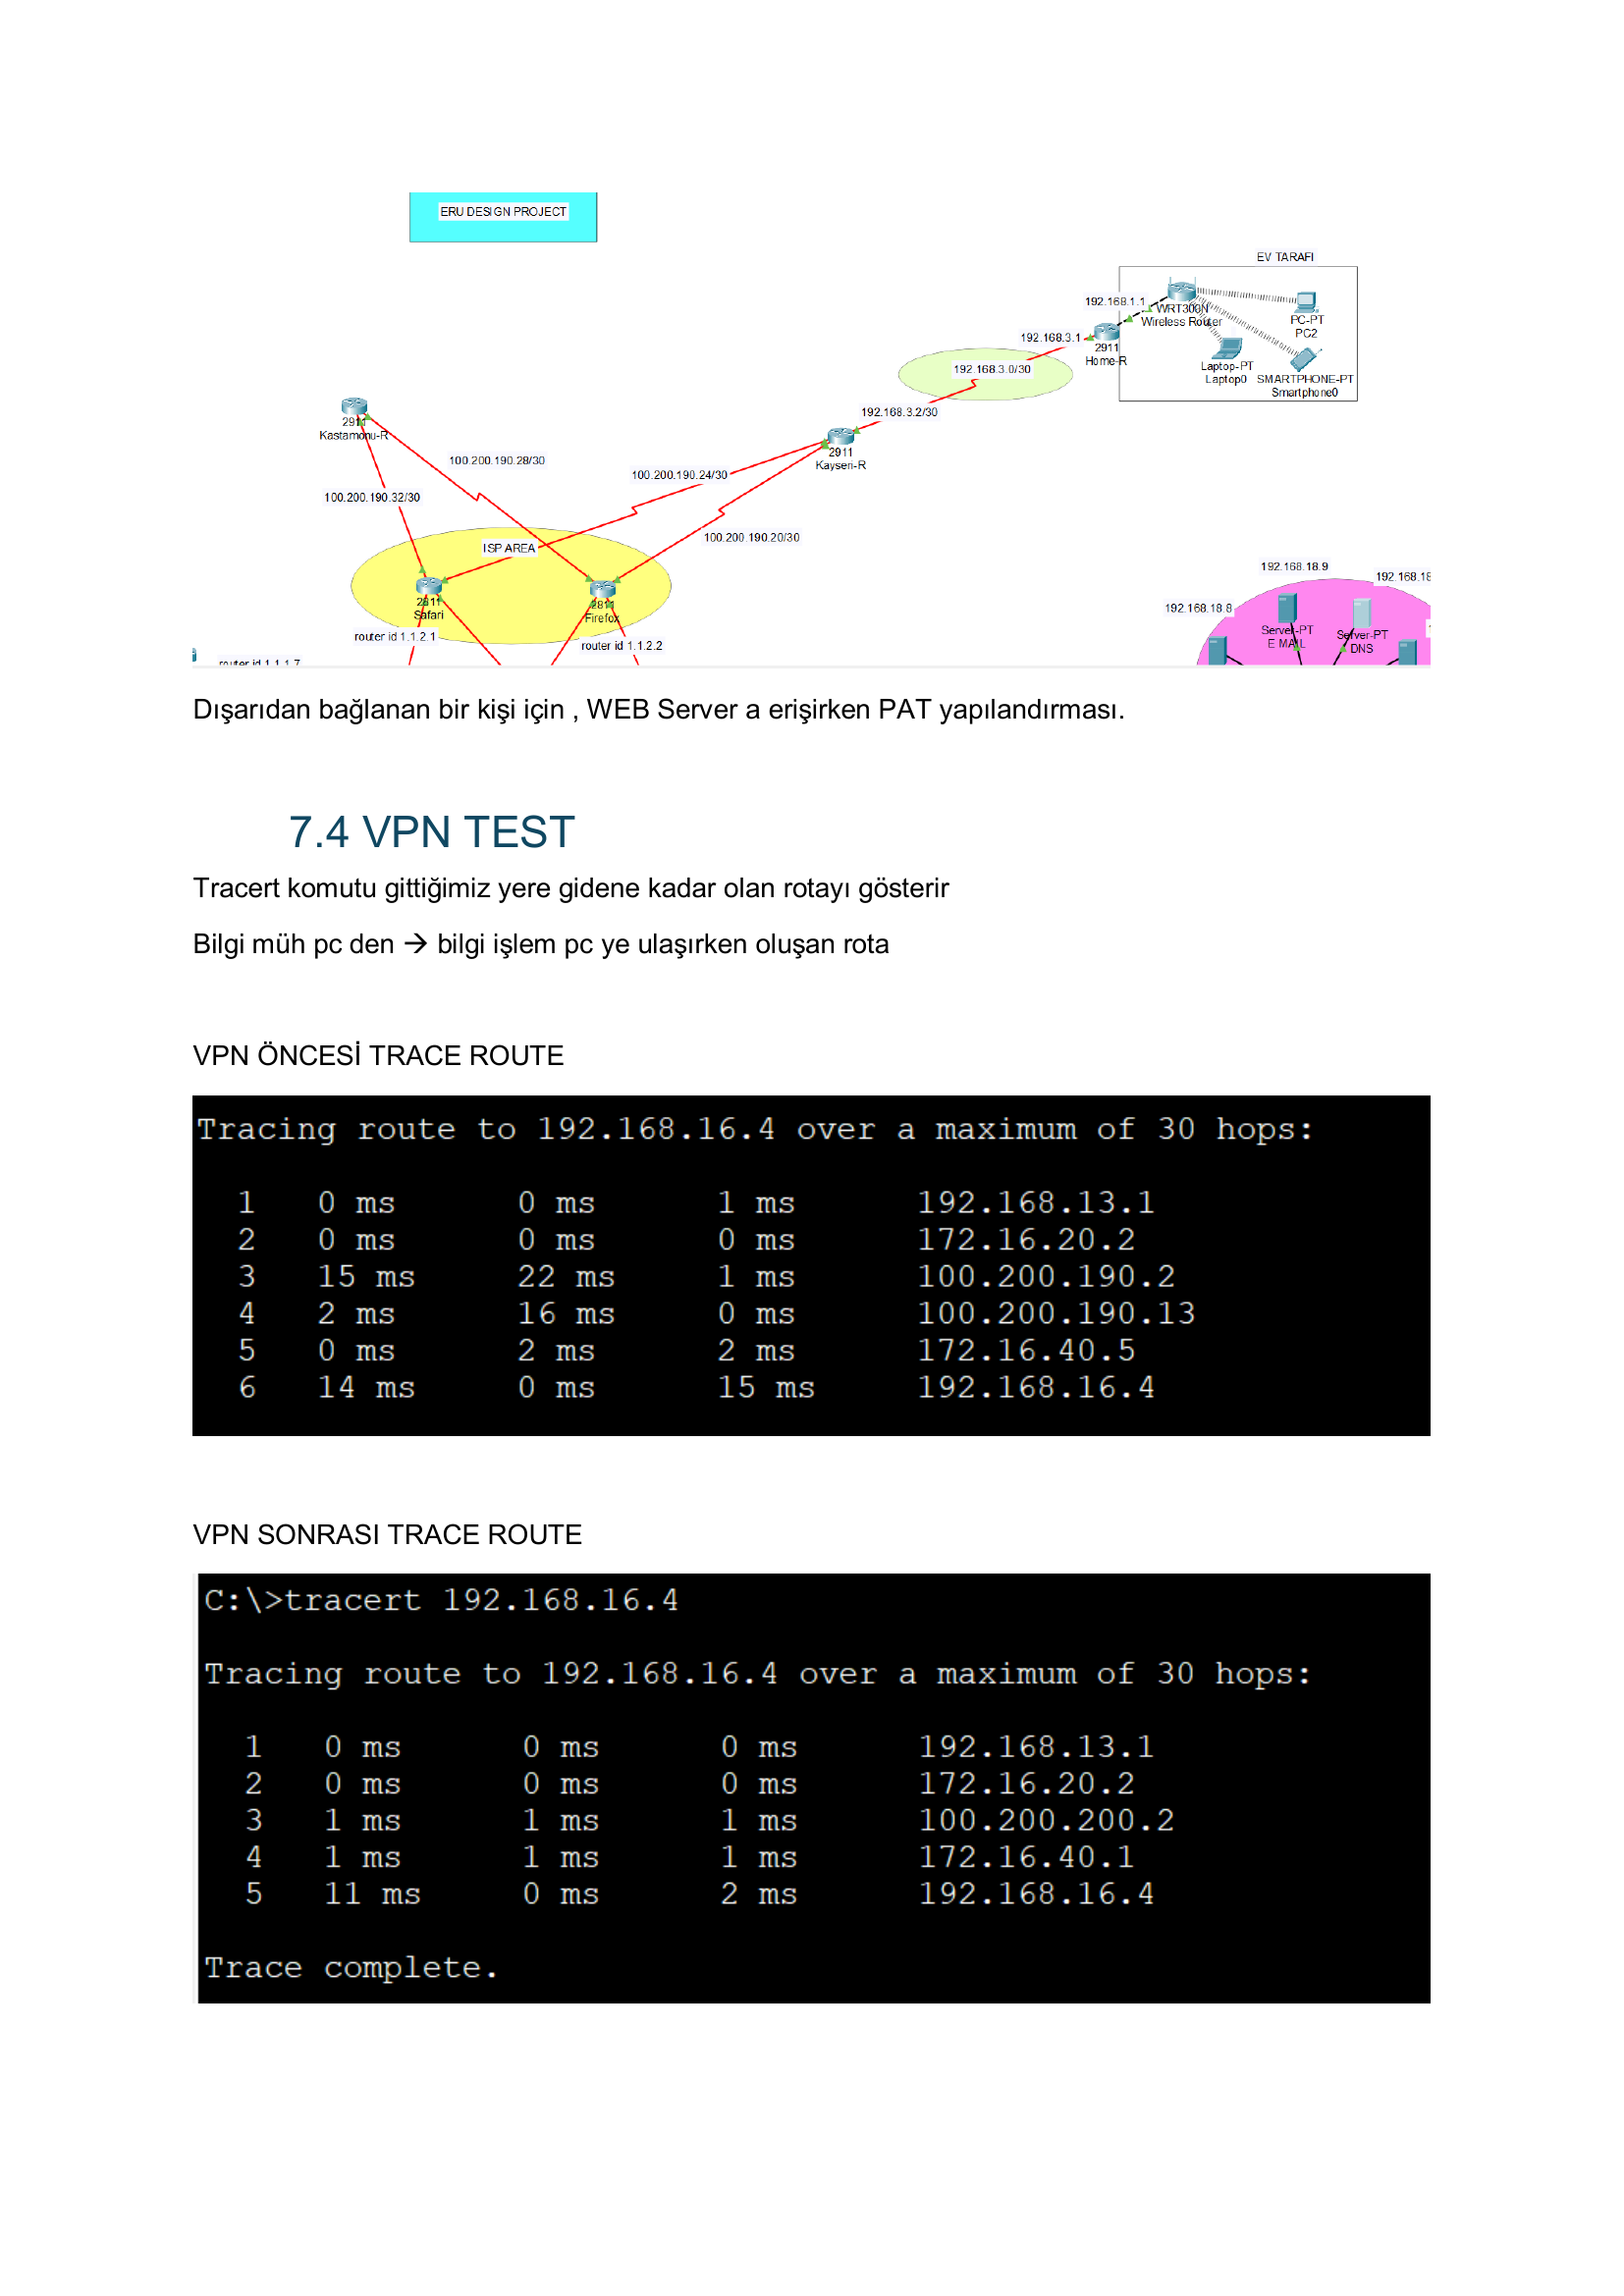
\includegraphics[width=0.85\textwidth]{figures/test-pat-vpn.png}
  \caption{PAT/NAT ve VPN Testi}
  \label{fig:test-vpn}
\end{figure}

\subsection{HSRP ve VoIP Testi}

HSRP aktif/standby durumu kontrol edilmiş ve VoIP hat numarası ataması doğrulanmıştır.

\begin{figure}[H]
  \centering
  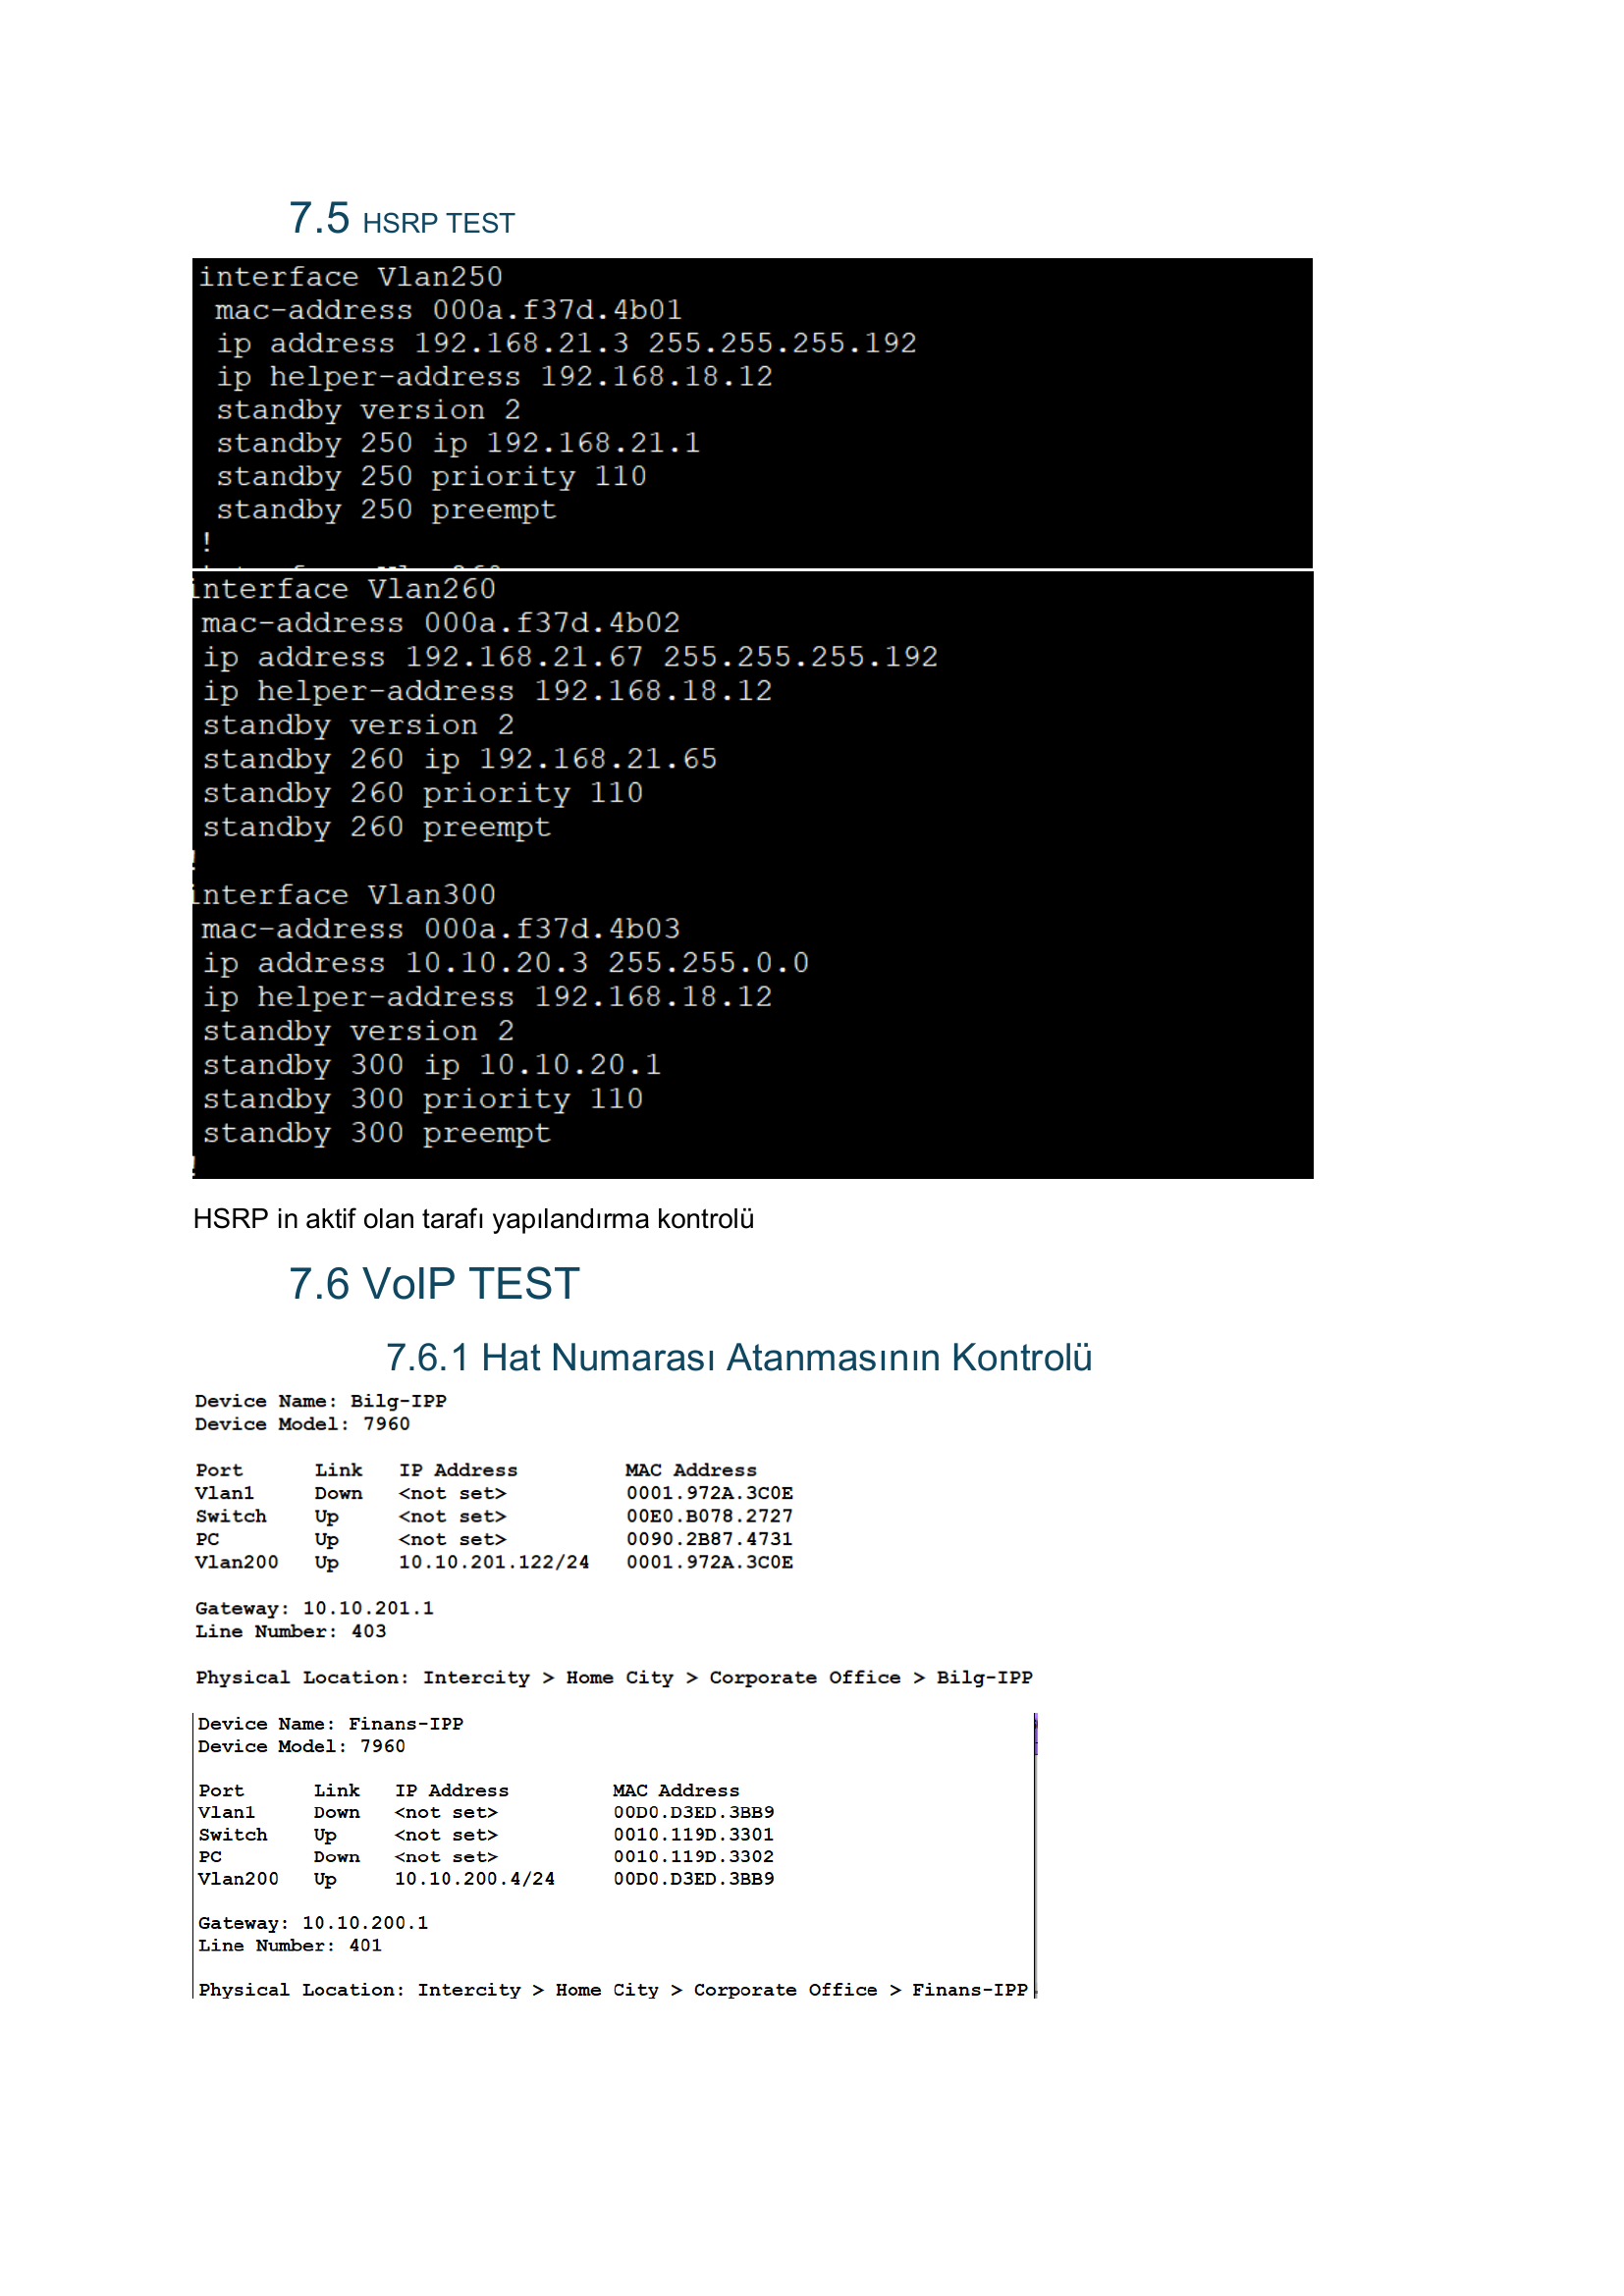
\includegraphics[width=0.85\textwidth]{figures/test-hsrp-voip.png}
  \caption{HSRP ve VoIP Testi}
  \label{fig:test-hsrp}
\end{figure}

\subsection{VoIP Arama ve ICMP Testi}

Fakülteler arası VoIP iletişimi ve ICMP (ping) testleri başarıyla gerçekleştirilmiştir.

\begin{figure}[H]
  \centering
  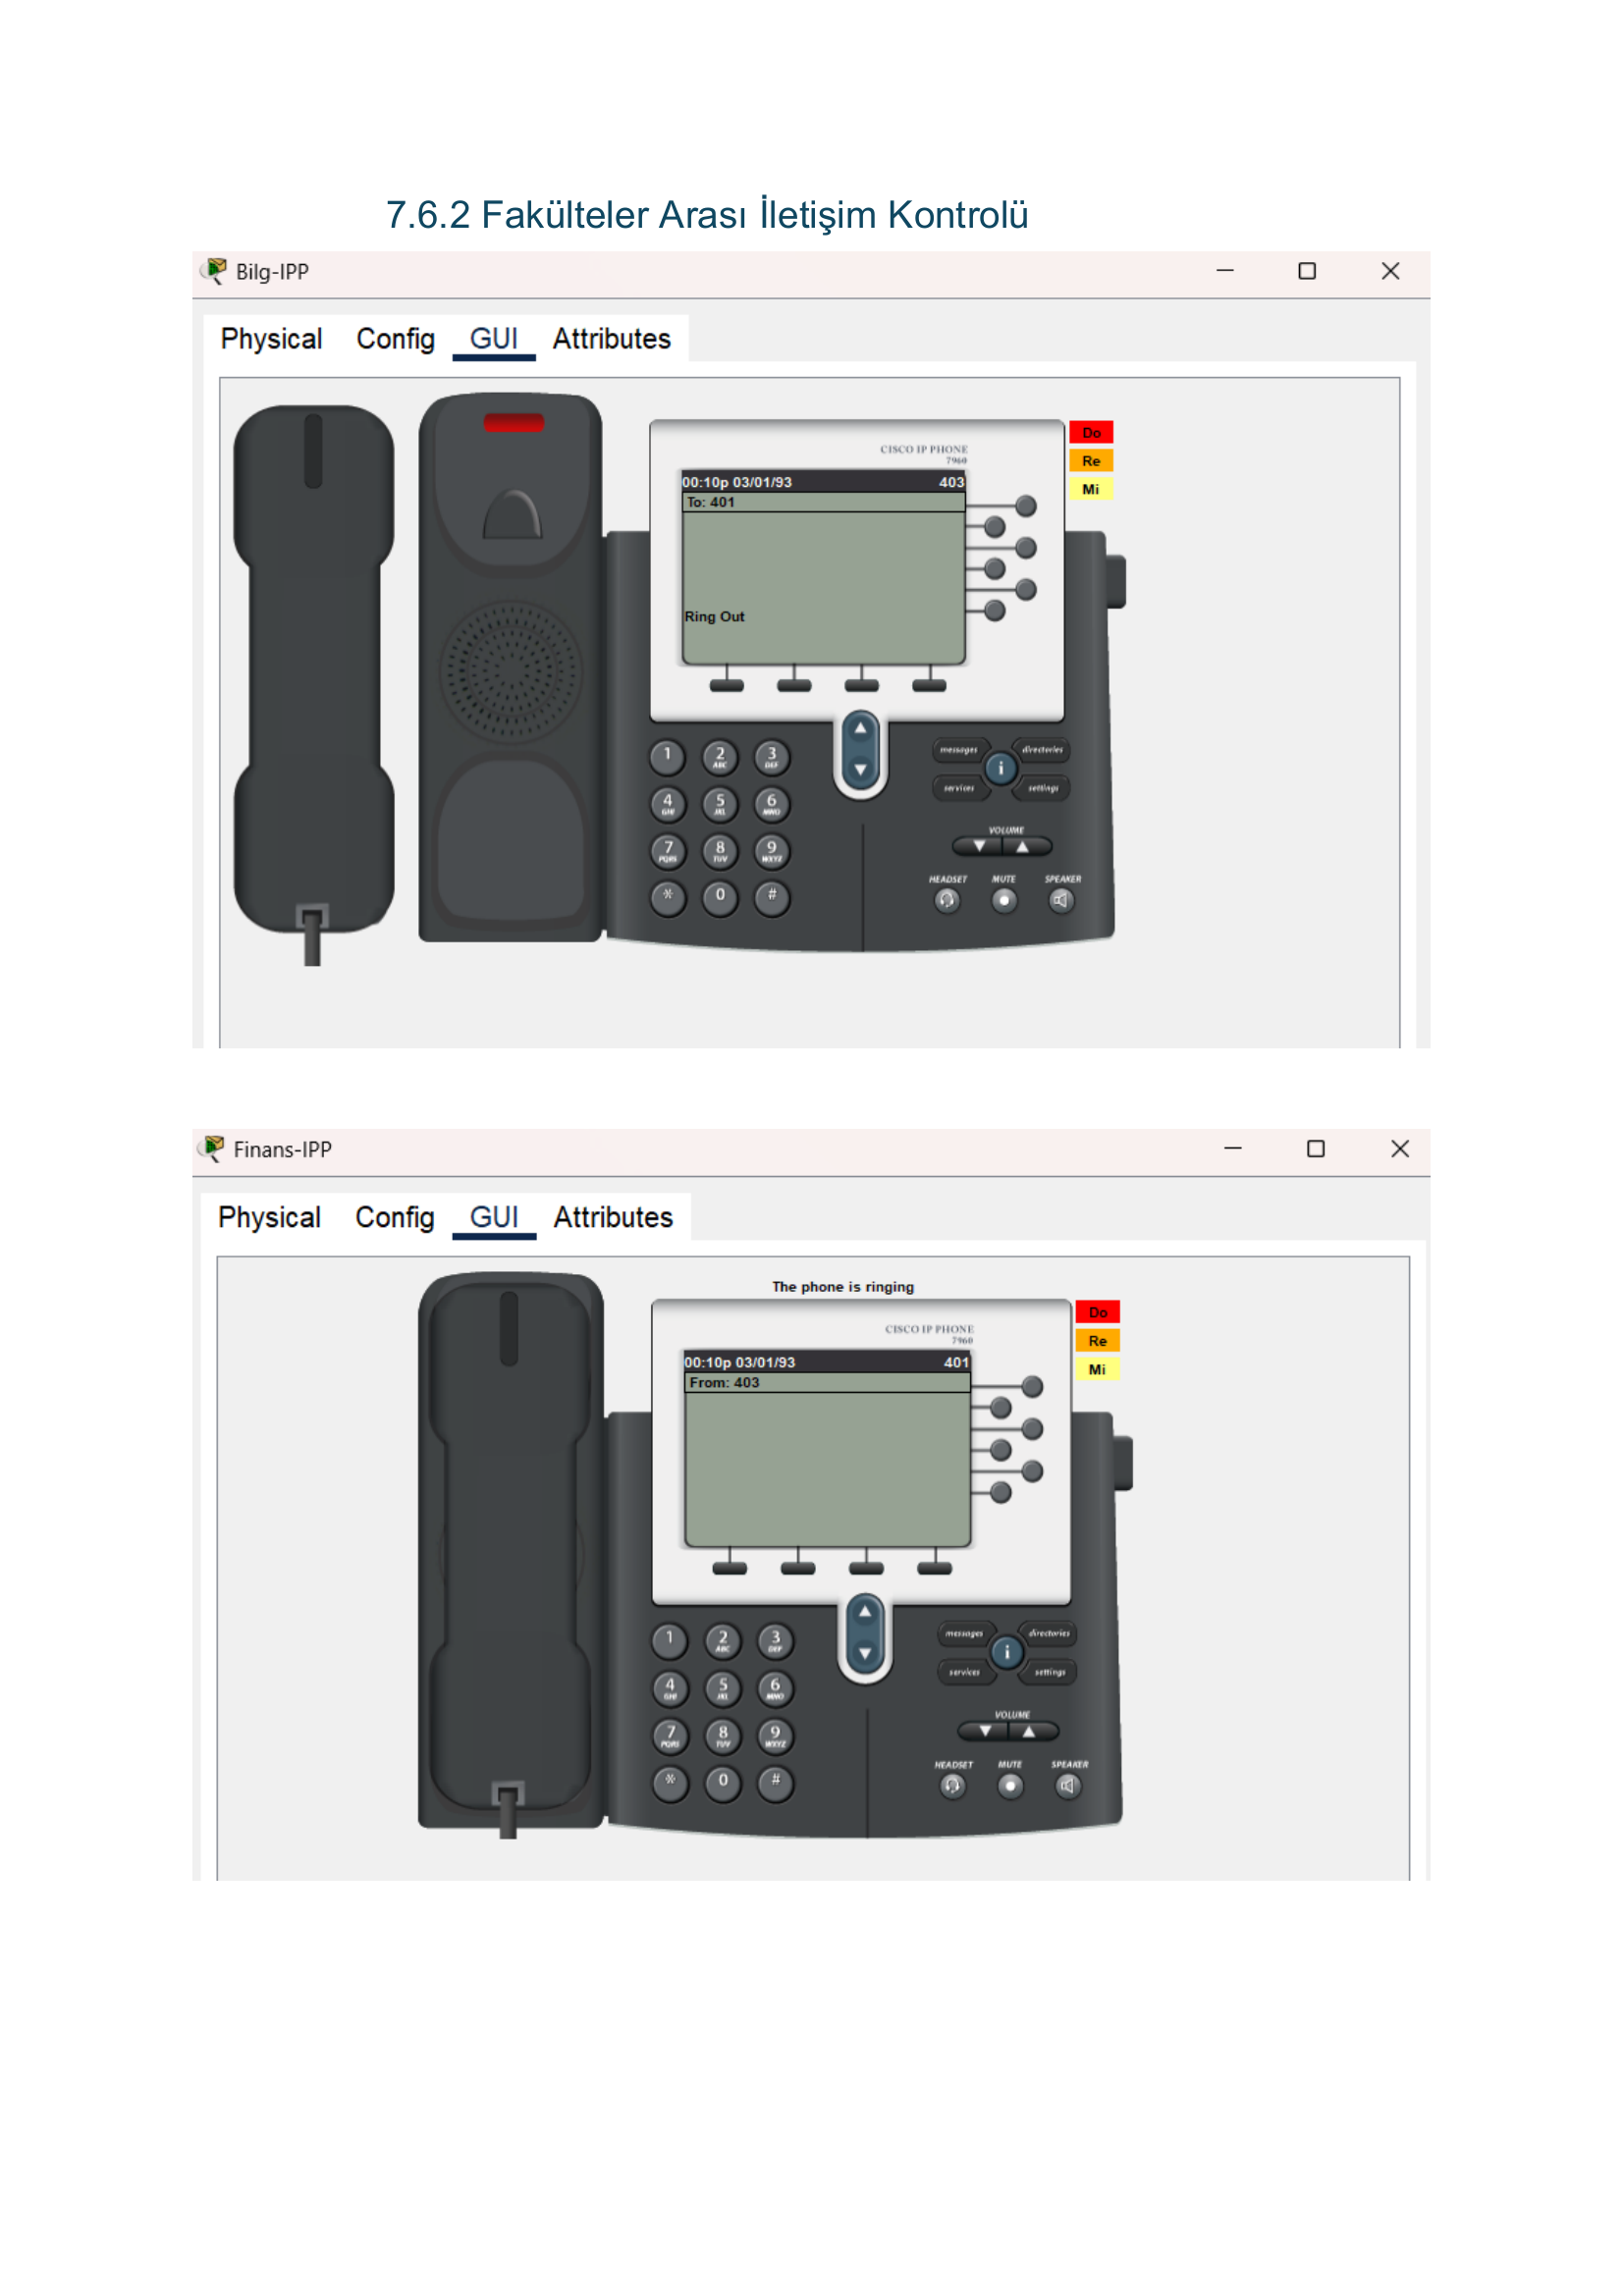
\includegraphics[width=0.85\textwidth]{figures/test-voip-icmp.png}
  \caption{VoIP Arama ve ICMP Testi}
  \label{fig:test-voip}
\end{figure}

\subsection{ICMP ve SSH Testi}

Fakülteler arası ICMP erişimi ve SSH ile uzaktan güvenli bağlantı kontrol edilmiştir.

\begin{figure}[H]
  \centering
  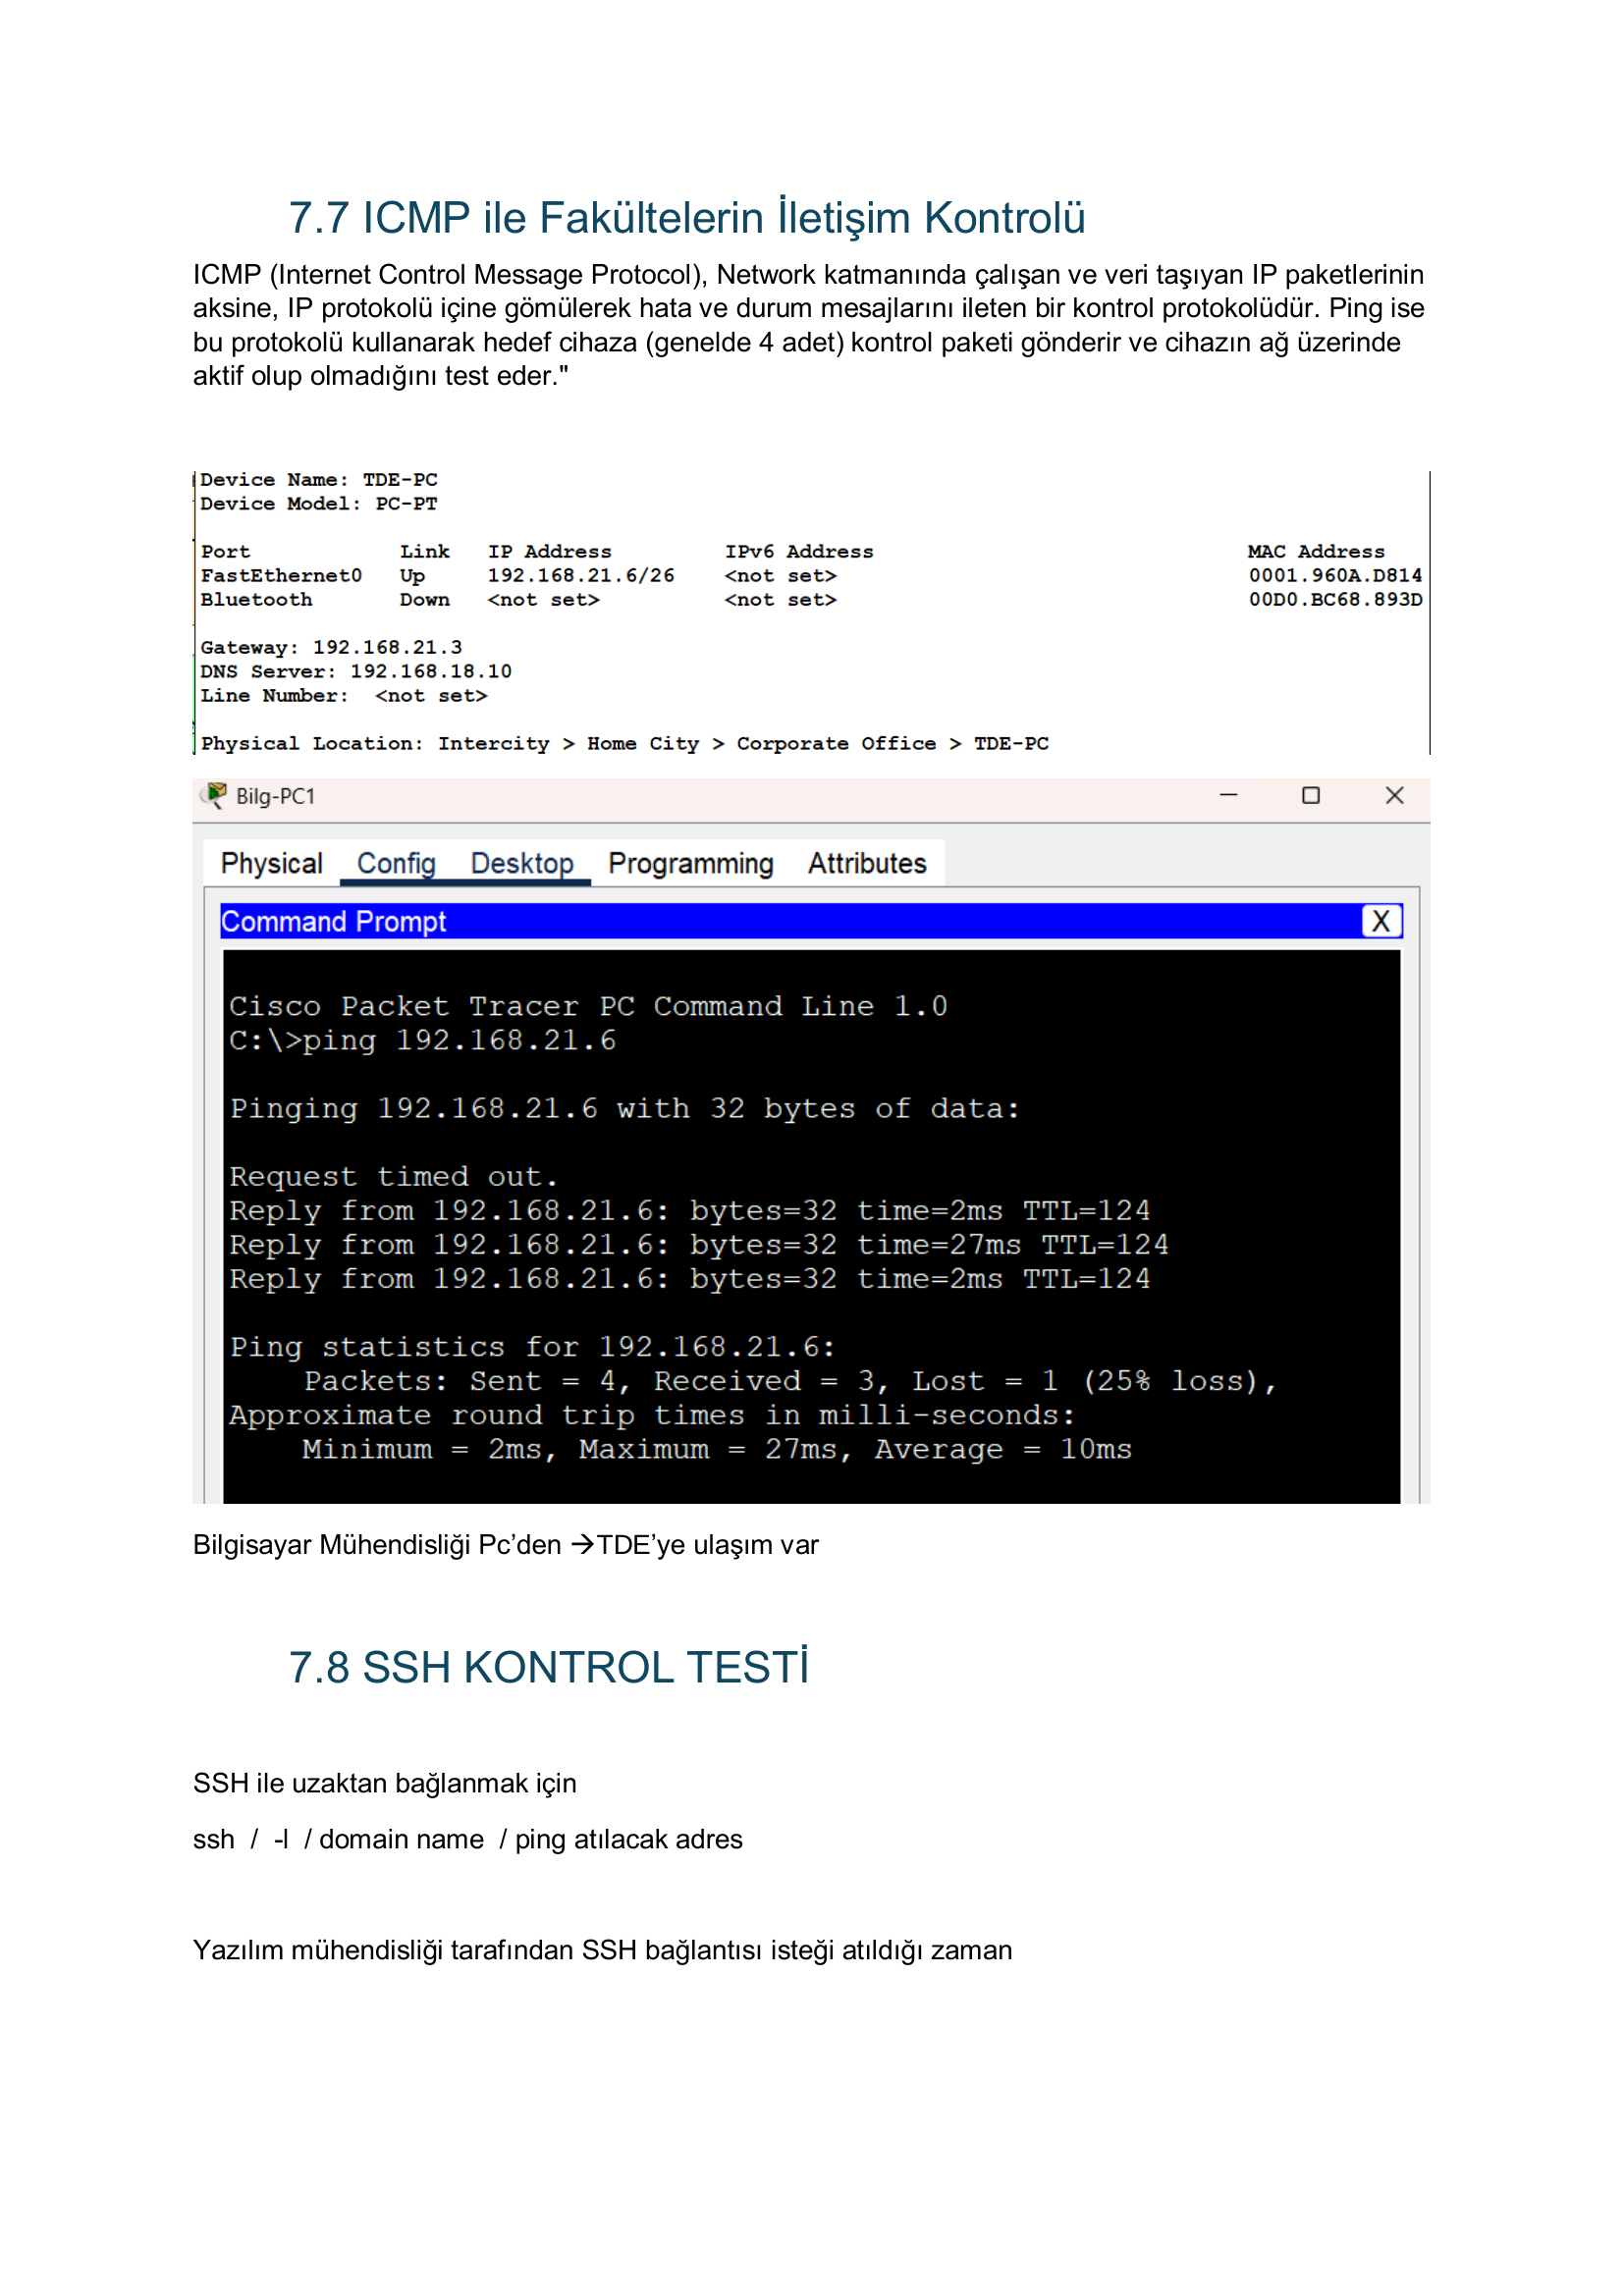
\includegraphics[width=0.85\textwidth]{figures/test-icmp-ssh.png}
  \caption{ICMP ve SSH Kontrol Testi}
  \label{fig:test-ssh}
\end{figure}

% =========================================
% 7. SONUÇ
% =========================================
\newpage
\section{Sonuç}

Bu proje kapsamında, bir üniversite kampüsünün ihtiyaç duyduğu tüm ağ gereksinimleri analiz edilmiş ve simülasyon ortamında başarıyla hayata geçirilmiştir.

\begin{infobox}[Temel Kazanımlar]
\begin{itemize}[noitemsep]
  \item \textbf{Yüksek Erişilebilirlik ve Süreklilik:} HSRP protokolü ve yedekli hatlar sayesinde, olası bir router veya hat arızasında bile ağın kesintisiz çalışmaya devam etmesi sağlanmıştır.
  \item \textbf{Güvenlik ve İzolasyon:} Fakülteler ve birimler VLAN yapısıyla mantıksal olarak birbirinden izole edilmiş, Site-to-Site VPN ile uzaktan güvenli erişim altyapısı kurulmuştur.
  \item \textbf{Yönetilebilirlik:} OSPF protokolü ile ağdaki değişikliklere hızlı adapte olunabilen, DHCP ile IP yönetiminin otomatikleştiği dinamik bir yapı oluşturulmuştur.
\end{itemize}
\end{infobox}

\vspace{1cm}

% --- TikZ: Summary Architecture ---
\begin{figure}[H]
\centering
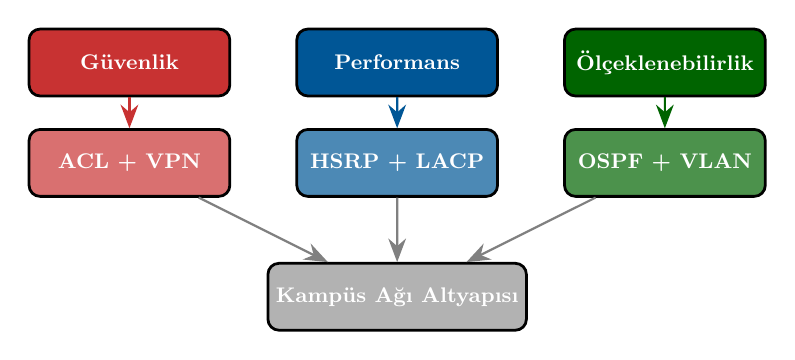
\begin{tikzpicture}[
  block/.style={draw, rounded corners, minimum width=3cm, minimum height=1cm, font=\small\bfseries, text=white, line width=1pt},
  arr/.style={-{Stealth[length=3mm]}, thick},
  scale=0.85, transform shape
]
  % Blocks
  \node[block, fill=corered] (sec) at (0,4) {Güvenlik};
  \node[block, fill=ciscoblue] (perf) at (4,4) {Performans};
  \node[block, fill=darkgreen] (scale) at (8,4) {Ölçeklenebilirlik};

  \node[block, fill=corered!70] (acl) at (0,2.5) {ACL + VPN};
  \node[block, fill=ciscoblue!70] (hsrp) at (4,2.5) {HSRP + LACP};
  \node[block, fill=darkgreen!70] (ospf) at (8,2.5) {OSPF + VLAN};

  \node[block, fill=gray!60] (campus) at (4,0.5) {Kampüs Ağı Altyapısı};

  % Arrows
  \draw[arr, corered] (sec) -- (acl);
  \draw[arr, ciscoblue] (perf) -- (hsrp);
  \draw[arr, darkgreen] (scale) -- (ospf);
  \draw[arr, gray] (acl) -- (campus);
  \draw[arr, gray] (hsrp) -- (campus);
  \draw[arr, gray] (ospf) -- (campus);
\end{tikzpicture}
\caption{Proje Mimari Özeti}
\label{fig:summary}
\end{figure}

Sonuç olarak; ölçeklenebilir, modern ve güvenli bir ağ topolojisi oluşturulmuş ve sistemin gerçek hayat senaryolarına uygunluğu test edilerek doğrulanmıştır.

\end{document}
